\chapter{Methods}
\label{ch:methods}


This chapter describes the graph inputs and graph-actor variants used in the
experiments. The presentation separates four design choices: feature scaling,
the base graph representation, substation-level augmentations, and graph
pooling.

\section{Input Scaling and Angle Representation}
\label{subsec:graph-feature-normalization}

This section collects everything that determines the numerical form of what the
encoder reads: two transformations applied to the continuous channels, and one
choice about how voltage angles are expressed in the first place. All three are
independent of the graph schema and of the grid.
Chapter~\ref{ch:wcci-transfer} measures their effect across two grids and
decides which of them to use; the mechanisms themselves are defined here.

\subsection{The two transformations}

Deterministic physical scaling is applied first, followed by optional running
standardization. Let $x_{i,f,t}$ be feature $f$ of node or edge
$i$ at time $t$. The complete pipeline is
\begin{align}
  x^{\mathrm{scale}}_{i,f,t}
  &=
  \begin{cases}
    x_{i,f,t}/s_f, & \text{if physical scaling is enabled},\\
    x_{i,f,t}, & \text{otherwise},
  \end{cases}
  \label{eq:graph-physical-scaling}\\
  \widehat{x}_{i,f,t}
  &=
  \begin{cases}
    \operatorname{clip}\!\left(
      \dfrac{x^{\mathrm{scale}}_{i,f,t}-\mu_{f,t}}
            {\sqrt{\sigma_{f,t}^{2}+\epsilon}},
      -c,c
    \right), & \text{if running normalization is enabled},\\
    x^{\mathrm{scale}}_{i,f,t}, & \text{otherwise}.
  \end{cases}
  \label{eq:graph-feature-normalization}
\end{align}
Here $s_f$ is a fixed physical reference and $\mu_{f,t}$ and
$\sigma_{f,t}^{2}$ are running moments estimated during training. When both
transformations are enabled, the moments describe $x/s_f$. Clipping applies
only to running standardization; $c=10$ by default and a non-positive value
disables clipping.

\subsection{Deterministic physical scaling}

Physical scaling divides each quantity by a constant with the same unit and
therefore preserves physical zero. Table~\ref{tab:graph-physical-scales} gives
the exact constants. The power base may be specified explicitly; otherwise the
largest installed generator rating is used,
with a 100~MW fallback when the environment does not expose generator ratings.
\\
\\
It is worth being explicit that this discards nothing within a grid. Division by
a fixed constant is invertible, so the mapping from megawatts to scaled units is
a bijection: the first linear layer can recover any function of the absolute
value it needs, and a load of $0.5$ on \texttt{bus14} is $70$~MW unambiguously.
The operation is a change of units, the same per-unit convention power systems
uses, adopted for the same reason. What it removes is the ability to compare
magnitudes \emph{across} grids, which is the intent: a transferable encoder
should respond to a load being half the largest unit's capacity rather than to
the number $200$. It is also the right target for the task, since whether a flow
is safe is set by its ratio to a thermal limit rather than by its absolute size
-- which is why the loading ratio needs no scaling at all.

\begin{table}[H]
  \centering
  \small
  \caption{Deterministic physical scales used for continuous graph features.}
  \label{tab:graph-physical-scales}
  \setlength{\tabcolsep}{5pt}
  \begin{tabular}{L{0.34\textwidth}L{0.25\textwidth}L{0.31\textwidth}}
    \toprule
    Features & Scale $s_f$ & Source \\
    \midrule
    \texttt{gen\_p}, \texttt{load\_p}, \texttt{p}
      & Power base in MW & Configured value or maximum generator rating. \\
    \texttt{gen\_theta}, \texttt{load\_theta}, \texttt{theta}
      & $180$ degrees & Fixed angular scale. \\
    \texttt{time\_before\_cooldown\_sub}
      & Maximum substation cooldown & Grid2Op environment parameter. \\
    \texttt{time\_before\_cooldown\_line}
      & Maximum line cooldown & Grid2Op environment parameter. \\
    \texttt{timestep\_overflow}
      & Allowed overflow duration & Grid2Op environment parameter. \\
    Maintenance time and duration
      & Episode horizon & Grid2Op chronic horizon. \\
    \bottomrule
  \end{tabular}
\end{table}

\subsection{Running standardization}

Running moments are estimated with Welford's online algorithm. One normalizer
is shared across agents and updated from the full state graph once per
environment step. Heterogeneous graphs maintain separate node statistics for
each node type. Edge statistics include only active physical-line relations;
inactive candidates and structural, asset-attachment, same-substation, and
virtual relations do not contribute.
\\
\\
The loading ratio \texttt{rho} is already dimensionless and is neither rescaled
nor standardized. Preserving it is also necessary when GCN uses \texttt{rho}
directly as a non-negative message weight. Binary connection states, node and
edge masks, domain masks, type indicators, and relation one-hot attributes are
also left unchanged. Only the continuous channels listed in
Table~\ref{tab:graph-physical-scales} enter the running statistics.
The running moments are frozen during evaluation.
\\
\\
\subsection{Angle representation}
\label{sec:line-node-angle}

Scaling cannot repair everything, because one channel is not well posed to begin
with. An absolute voltage angle is measured against whichever bus is chosen as
slack, so its level is a property of that reference rather than of the grid
state, and only differences between angles carry physical meaning. Line flow
depends on the difference across the line. Dividing by a constant moves both
grids together and leaves any displacement between them untouched, so no choice
of scale addresses it.
\\
\\
The alternative is to carry the angle as the drop along each line,
\[
  \Delta\theta_{\ell} \;=\; \theta^{\,\mathrm{or}}_{\ell} - \theta^{\,\mathrm{ex}}_{\ell},
\]
which is what \texttt{gnn\_angle\_representation = "edge\_diff"} selects. It is
gauge-invariant by construction, since adding a constant to every angle leaves
it unchanged, and it is dense, since every line has two ends whereas a busbar
carries an angle only when an asset is attached to it. The absolute per-asset
channels are removed when it is enabled, because keeping them would preserve
exactly the reference dependence the change exists to remove.
\\
\\
Gauge invariance matters beyond comparing grids. In a decentralized setting the
slack reference is global, so under absolute angles an event on the far side of
the grid that does not affect an agent still moves all of its angle inputs. The
drop is a property of one line.
\\
\\
Where the channel lives depends on how the representation models a line.

\begin{table}[H]
  \centering
  \small
  \caption{Where the voltage angle enters each representation, under the two
  ways of expressing it.}
  \label{tab:angle-placement}
  \setlength{\tabcolsep}{4pt}
  \begin{tabular}{L{0.26\textwidth}L{0.30\textwidth}L{0.34\textwidth}}
    \toprule
    Representation & Absolute angle & Angle drop \\
    \midrule
    Busbar & On busbar nodes, averaged over the attached assets &
    On the physical line edge \\
    Disaggregated & On generator and load nodes &
    On the physical line edge \\
    Disaggregated with line nodes & On generator and load nodes &
    On the \emph{line node} \\
    \bottomrule
  \end{tabular}
\end{table}

\subsubsection{The explicit-line graph}

In the busbar and disaggregated representations a line is an edge, so the drop
has an obvious home and simply moves from the node features onto that edge. The
explicit-line representation of Section~\ref{sec:heterogeneous-line-graph}
inverts the arrangement: each line is a node carrying its own loading, status,
overflow and cooldown, and the remaining edges are busbar-to-line attachments
that carry no physical channel at all, only a relation type. There is no edge
for the drop to move onto.
\\
\\
It is therefore written on the line node itself, in the column the absolute
angle previously occupied. This keeps the line node's description of its own
line complete: loading, status, cooldown, and now the angle across it, which is
the quantity that drives the flow the loading measures. Handling this case
explicitly matters because the failure would otherwise be silent -- the generic
correction removes the absolute angle from the node features and adds the drop
to the edge features, and in a schema whose edge block is empty the first half
applies while the second has nowhere to land, leaving an observation with no
angle information at all.
\\
\\
The gain is largest exactly where the absolute channel was thinnest. Under
absolute angles an actor reads them only through the generators and loads it
owns, while the line nodes -- which carry loading, status and cooldown -- carry
no angle. On \texttt{bus14}, agent 1 sees three angle values in total, two of
which are duplicates, because a generator and a load on the same busbar read the
same bus angle.

\begin{table}[H]
  \centering
  \small
  \caption{Local-graph rows carrying an angle on \texttt{bus14}, explicit-line
  representation without one-hop context.}
  \label{tab:angle-coverage}
  \setlength{\tabcolsep}{6pt}
  \begin{tabular}{lccc}
    \toprule
    Agent & Nodes & Absolute angle & Angle drop \\
    \midrule
    0 & 22 & 5 \; (23\,\%) & 8 \; (36\,\%) \\
    1 & 20 & 3 \; (15\,\%) & 8 \; (40\,\%) \\
    2 & 29 & 8 \; (28\,\%) & 9 \; (31\,\%) \\
    \bottomrule
  \end{tabular}
\end{table}

Every row counted in the angle-drop column is a line node, so each agent holds
the drop across every line it touches, including the boundary lines whose far
endpoint the leakage-free construction deliberately omits. That is new
information relative to the absolute angle, and it is of the same kind as the
loading already carried by those line nodes: a measurement of a line the agent
is attached to, not a state of equipment it cannot see.

\subsubsection{Masking on outage}

The drop has to be zeroed when a line is out. The simulator zeroes the loading
of a disconnected line but leaves its endpoint angles at their last solved
values, so an unmasked drop reports a confident number on a dead line while
every other channel on the same row reports that it is dead. Measured on
\texttt{bus14}, a line taken out of service kept endpoint angles of $-1.06$ and
$-7.62$ degrees, a spurious drop of $6.56$, alongside a loading of exactly zero.
The line-node channel is therefore masked by line status explicitly. The busbar
and disaggregated representations need no equivalent step, because an inactive
edge is zeroed in full before message passing.

\subsubsection{What is unchanged}

In the explicit-line graph the drop replaces the absolute angle rather than
joining it, so the node feature width, the column position, and the encoder
input dimension are all unchanged; attachment edges remain free of physical
channels. In the other two representations the node block loses the angle
columns and the physical line edge gains one
(Table~\ref{tab:angle-feature-dims}). In every case message passing, graph
readout, and candidate-action scoring are untouched, and keeping the absolute
angle reproduces the previous observation exactly, so runs predating this option
remain a valid control.

\begin{table}[H]
  \centering
  \small
  \caption{Feature dimensions under the two ways of expressing the angle, at the
  default edge-feature schema version. The explicit-line graph keeps both widths
  because the drop replaces the absolute angle in the same node column rather
  than moving to an edge.}
  \label{tab:angle-feature-dims}
  \setlength{\tabcolsep}{8pt}
  \begin{tabular}{llrr}
    \toprule
    Graph type & Angle carried as & Node width & Edge width \\
    \midrule
    \texttt{bus} & Absolute & 6 & 4 \\
    \texttt{bus} & Drop & 4 & 5 \\
    \texttt{heterogeneous} & Absolute & 8 & 10 \\
    \texttt{heterogeneous} & Drop & 7 & 11 \\
    \texttt{heterogeneous\_line} & Absolute & 13 & 9 \\
    \texttt{heterogeneous\_line} & Drop & 13 & 9 \\
    \bottomrule
  \end{tabular}
\end{table}

\subsection{Use across the experiments}

All three choices are available to every experiment. The screening protocol of
Chapter~\ref{ch:experiments} and the sparse-control experiments of
Chapter~\ref{ch:sparse-control} use none of them and read raw features. The
transfer study of Chapter~\ref{ch:wcci-transfer} enables physical scaling and
the angle drop, and deliberately leaves running standardization off:
Section~\ref{sec:wcci-running-norm} measures it on a cross-grid comparison and
finds it counterproductive for features whose support is sparse, because
standardizing a channel that is mostly structural zeros relocates that point
mass to a grid-dependent value.


\section{Graph Representations}
\label{sec:graph-representation}

The graph observation can use one of three base representations. The
\texttt{bus} representation aggregates equipment values onto busbar nodes. The
\texttt{heterogeneous} representation disaggregates generators and loads into
explicit asset nodes while keeping physical lines as busbar-to-busbar edges. The
\texttt{heterogeneous\_line} representation further disaggregates transmission
lines into explicit line nodes.
\\
\\
Table~\ref{tab:schema-comparison} states what separates them. The node schema
also determines how a boundary transmission line is represented in a local
actor graph. Consequently, the three representations are not
information-equivalent: they expose different amounts of context about the
substation at the far end of a shared line. This distinction is made explicit
in Section~\ref{subsec:graph-local-global}.

\begin{table}[H]
  \centering
  \scriptsize
  \caption{The three graph schemas. Each row is a consequence of how much
  equipment receives its own node.}
  \label{tab:schema-comparison}
  \setlength{\tabcolsep}{4pt}
  \begin{tabular}{L{0.15\textwidth}L{0.24\textwidth}L{0.24\textwidth}L{0.25\textwidth}}
    \toprule
    Aspect & \texttt{bus} & \texttt{heterogeneous} & \texttt{heterogeneous\_line} \\
    \midrule
    Node types & Busbar & Busbar, generator, load & Busbar, generator, load, transmission line \\
    Generator and load state & Summed and averaged onto the busbar & One node per asset & One node per asset \\
    Physical line & Direct busbar-to-busbar edge & Typed direct busbar-to-busbar edge & Typed node between its endpoint busbars \\
    Line state & Continuous edge attributes & Continuous edge attributes & Features of the line node \\
    Minimum useful depth & One layer for adjacent busbar exchange & One layer for adjacent busbars; two for asset-to-remote-busbar flow & Two layers for adjacent busbar exchange through a line node \\
    Hidden line state & None: the edge modifies a message & None: the edge modifies a message & Yes: each line obtains and updates an embedding \\
    Far-end context in a local actor graph & Live neighboring busbar, including aggregated power and angle & Live neighboring busbar, but no neighboring generator or load nodes & None; the shared line node replaces the need for a far-end busbar \\
    Node count & $SB$ & $SB+N_g+N_d$ & $SB+N_g+N_d+L$ \\
    \bottomrule
  \end{tabular}
\end{table}

\subsection{Candidate graph and dynamic mask}
\label{subsec:graph-candidate-edges}

All three schemas share one construction.
\\
\\
Grid2Op exposes the instantaneous electrical state and topology through a
structured observation~\cite{donnot2020grid2op}. For each representation,
the graph construction keeps the set of candidate nodes and edges fixed
throughout an episode while using a dynamic edge mask to express the topology
that is electrically active at time step~$t$.
\\
\\
For agent~$a$, the graph observation can be written as
\begin{equation}
  \mathcal{G}^{(a)}_t =
  \left(\mathcal{V}^{(a)},\mathcal{E}^{(a)}_{\mathrm{cand}},
  \mathbf{X}^{(a)}_t,\mathbf{Z}^{(a)}_t,
  \mathbf{m}^{(a)}_t,\mathbf{n}^{(a)}_t,
  \mathbf{c}^{(a)}\right),
  \label{eq:agent-graph-observation}
\end{equation}
where $\mathcal{V}^{(a)}$ and
$\mathcal{E}^{(a)}_{\mathrm{cand}}$ are static, $\mathbf{X}^{(a)}_t$ contains
node features, $\mathbf{Z}^{(a)}_t$ contains edge features,
$\mathbf{m}^{(a)}_t$ indicates which candidate edges are active,
$\mathbf{n}^{(a)}_t$ marks currently visible nodes, and
$\mathbf{c}^{(a)}$ marks nodes belonging to the agent's controlled domain.
The controlled mask is static, whereas the edge and visibility masks change
with line status and busbar assignments. This separates the fixed candidate
layout from the electrical topology that can change after every action.
\\
\\
The mechanism is easiest to see on a transmission line in the \texttt{bus} and
\texttt{heterogeneous} schemas, where a physical line is an edge. Consider a
line~$\ell$ whose origin and extremity
belong to substations $o(\ell)$ and $e(\ell)$. For every pair of possible
endpoint busbars $(b_o,b_e)$, the graph reserves the two directed candidate
edges
\begin{equation}
  i(o(\ell),b_o)\rightarrow i(e(\ell),b_e)
  \quad\text{and}\quad
  i(e(\ell),b_e)\rightarrow i(o(\ell),b_o),
  \label{eq:candidate-line-edges}
\end{equation}
so each physical line contributes $2B^2$ candidate directed edges and the two
directions share the same line attributes. For the usual case $B=2$, one line
reserves eight candidate edges even though at most two, one per direction, are
electrically active at any time.
\\
\\
Which of them is active is decided by the mask
\begin{equation}
  m_{\ell,b_o,b_e,t}=
  \mathbf{1}\!\left[\text{line }\ell\text{ is connected at }t\right]
  \mathbf{1}\!\left[b^{\mathrm{or}}_{\ell,t}=b_o\right]
  \mathbf{1}\!\left[b^{\mathrm{ex}}_{\ell,t}=b_e\right].
  \label{eq:physical-edge-mask}
\end{equation}
A disconnected line has all of its candidates masked; a connected one keeps
only the pair matching its current origin and extremity busbars, provided both
endpoint nodes are visible. A topology action therefore changes connectivity
by changing $\mathbf{m}^{(a)}_t$, never by rebuilding the graph, and the node
and edge tensors keep a fixed shape for the whole episode. The same candidate
and mask pattern governs the asset attachments of
Section~\ref{sec:heterogeneous-graph-representation} and the line-node
attachments of Section~\ref{sec:heterogeneous-line-graph};
Appendix~\ref{app:graph-construction} gives the resulting sizes and the
masking conventions.

{\color{clarif}
\paragraph{Why a fixed shape rather than rebuilding the graph.}
Rebuilding the graph after every topology action would be the more obvious
implementation, and it is rejected for four reasons, the last of which is the
substantive one.
\begin{enumerate}
  \item \textbf{The interface requires it.} Each agent's observation is declared
  once as a fixed-size space, and rollouts are collected from many environments
  stepping in parallel. The rollout buffer is allocated once, from the shape of
  the first observation, and written into at every step; an observation whose
  node or edge count changed mid-episode could neither be stacked across
  environments nor stored in that buffer.
  \item \textbf{Batching stays trivial.} A fixed layout means node and edge
  tensors for different environments, agents and time steps are stacked by
  concatenation, and the message-passing index is built once and reused, rather
  than a variable-size graph being assembled and re-indexed on every forward
  pass.
  \item \textbf{Row identity is stable.} Row $i$ always denotes the same
  physical busbar, line or asset. The candidate-action head of
  Section~\ref{sec:candidate-action-scoring} depends on this directly: it maps
  each discrete action to the graph rows it modifies once, before training. If
  the node set were rebuilt per step, that mapping would have to be recomputed
  at every step and would refer to different objects at different times.
  \item \textbf{Absent connections stay visible.} A rebuilt graph would contain
  only the connections that currently exist, which hides the ones an action
  could create: the empty busbar an element would be moved onto would simply not
  be in the graph, so no encoder reading it could evaluate that action. Keeping
  the candidate set fixed means the reachable topologies are present as masked
  structure, and the mask makes the current topology an explicit input rather
  than something inferable only from which messages happen to exist. This is the
  busbar information asymmetry identified by~\textcite{dejong2025gnntopo}.
\end{enumerate}
The cost is memory. With $B=2$ a line reserves eight directed candidates of
which at most two are ever active, so the edge tensor is roughly four times
larger than the active topology requires. On the grids used here that is
affordable, and Appendix~\ref{app:graph-construction} gives the exact sizes.
}
\\
\\
The following subsections define the three schemas.

\subsection{Busbar Representation}
\label{subsec:busbar-representation}

The \texttt{bus} schema is the compact busbar representation. Busbars are the
only nodes, active transmission lines form the graph edges, and generator and
load quantities are aggregated into their currently assigned busbars.

\begin{figure}[htbp]
  \centering
  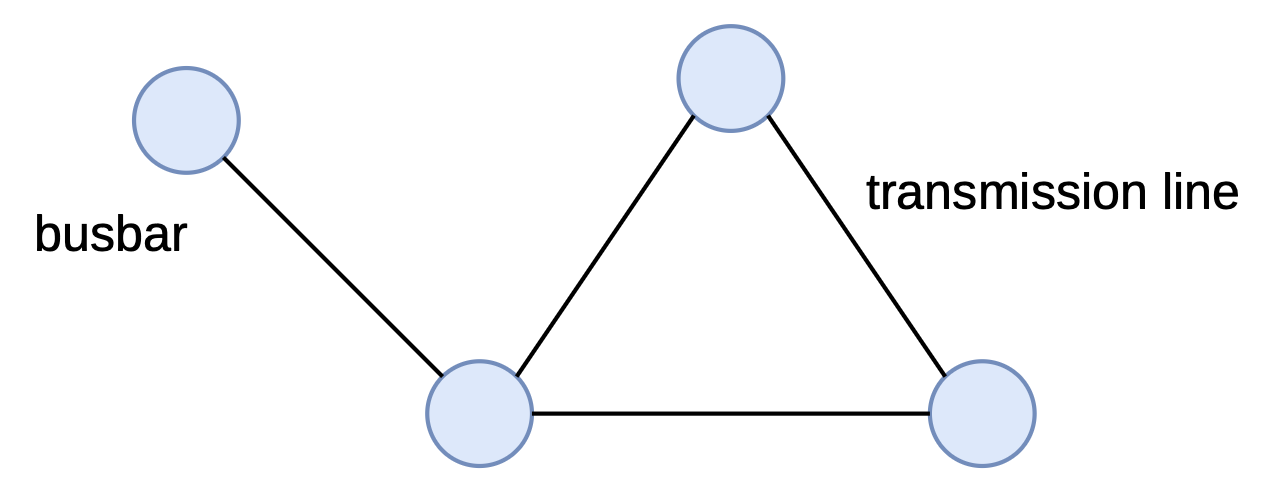
\includegraphics[width=0.94\linewidth]{figures/graph_busbar_baseline.png}
  \caption{Busbar graph representation. Blue nodes denote busbars and black
  connections denote active transmission-line relations. Generator and load
  quantities are aggregated into the features of their associated busbars.}
  \label{fig:busbar-graph-representation}
\end{figure}

\subsubsection{Nodes and features}
\label{subsec:graph-busbar-nodes}

Let $S$ denote the number of substations and let $B$ denote the maximum number
of busbars per substation. A node is created for every substation--busbar pair,
including busbars to which no asset is connected at the current time. A global
node identifier is assigned as
\begin{equation}
  i(s,b)=sB+b,
  \qquad s\in\{0,\ldots,S-1\},\quad
  b\in\{0,\ldots,B-1\}.
  \label{eq:busbar-node-id}
\end{equation}
The complete graph therefore contains $SB$ nodes.
\\
\\
Table~\ref{tab:graph-node-features} lists the six node features. Generator and
load quantities are assigned to the
busbar specified by the current topology vector. Active powers are summed when
several assets occupy the same busbar, whereas the corresponding angles are
averaged. Disconnected assets do not contribute to any node. The substation
cooldown is repeated on every busbar node of that substation.

\begin{table}[H]
  \centering
  \small
  \caption{Features attached to each busbar node.}
  \label{tab:graph-node-features}
  \setlength{\tabcolsep}{5pt}
  \begin{tabular}{L{0.28\textwidth}L{0.62\textwidth}}
    \toprule
    Feature & Definition \\
    \midrule
    \texttt{gen\_p} & Sum of active generator power connected to the busbar. \\
    \texttt{gen\_theta} & Mean voltage angle of generators connected to the busbar. \\
    \texttt{load\_p} & Sum of active load power connected to the busbar. \\
    \texttt{load\_theta} & Mean voltage angle of loads connected to the busbar. \\
    \texttt{time\_before\_cooldown\_sub} & Remaining substation cooldown. \\
    \texttt{domain\_mask} & One for a substation controlled by the agent and zero for a contextual neighbor. \\
    \bottomrule
  \end{tabular}
\end{table}

\noindent This aggregation produces a compact representation but deliberately removes
the identities and counts of individual generators and loads.

\subsubsection{Relations and edge features}
\label{subsec:graph-line-edge-features}

The only physical relations (edges) of the busbar schema are the busbar-to-busbar transmission line.
The dynamic attributes copied onto active physical-line edges are given in
Table~\ref{tab:graph-edge-features}. The two maintenance features are present
only for environments with scheduled maintenance.

\begin{table}[H]
  \centering
  \small
  \caption{Features attached to physical-line edges.}
  \label{tab:graph-edge-features}
  \setlength{\tabcolsep}{5pt}
  \begin{tabular}{L{0.32\textwidth}L{0.58\textwidth}}
    \toprule
    Feature & Definition \\
    \midrule
    \texttt{line\_status} & Binary connection status of the physical line. \\
    \texttt{rho} & Line loading relative to its thermal limit. \\
    \texttt{timestep\_overflow} & Number of consecutive time steps in overload. \\
    \texttt{time\_before\_cooldown\_line} & Remaining cooldown before another line action is legal. \\
    \texttt{time\_next\_maintenance} & Time until scheduled maintenance, when available. \\
    \texttt{duration\_next\_maintenance} & Duration of scheduled maintenance, when available. \\
    \bottomrule
  \end{tabular}
\end{table}

\noindent The edge embedding of a busbar-to-busbar transmission edge is
exactly the row of Table~\ref{tab:graph-edge-features}. \hl{Optional
same-substation edges use the same feature width: all physical channels are
zero except \texttt{rho}$=1$, which is a neutral structural value. The
homogeneous schema does not append relation one-hots, so these optional
relations are distinguished only by their endpoints and neutral physical
attributes.}

\subsubsection{Local information boundary}

For an agent-local \texttt{bus} graph, all busbars of controlled substations
are present. A live boundary line additionally requires exactly one contextual
node: the far-end busbar to which that line is currently attached. This node is
needed because the shared line is an edge, and both endpoint nodes must exist
for its features to reach the controlled busbar through message passing.
Because generator and load quantities are aggregated onto busbars, the visible
far-end busbar also exposes aggregated neighboring \texttt{gen\_p},
\texttt{load\_p}, and angle features. The other busbar candidates at that
neighboring substation are masked, even if they carry generation or load. If
the boundary line is disconnected, no neighboring busbar remains visible.

% \subsubsection{Message-passing path}
% \label{subsec:graph-busbar-message-path}

% Asset values already sit on their busbar, so information follows the single
% path busbar $\leftrightarrow$ busbar and one message-passing layer is enough to
% carry a substation's state to an adjacent one. This is the shortest path of the
% three schemas, and the baseline against which the two disaggregated ones trade
% extra hops for individually addressable equipment.


\subsection{Disaggregated Representation}
\label{sec:heterogeneous-graph-representation}

The \texttt{heterogeneous} schema keeps busbars as the backbone and adds one node
per generator and load. Transmission lines remain busbar-to-busbar edges. The
node set is
\begin{equation}
  \mathcal{V} =
  \mathcal{V}_{\mathrm{bus}}
  \cup \mathcal{V}_{\mathrm{gen}}
  \cup \mathcal{V}_{\mathrm{load}},
  \label{eq:heterogeneous-node-set}
\end{equation}
with typed directed relations between these sets. Generator and load states are
therefore preserved individually.

\begin{figure}[H]
  \centering
  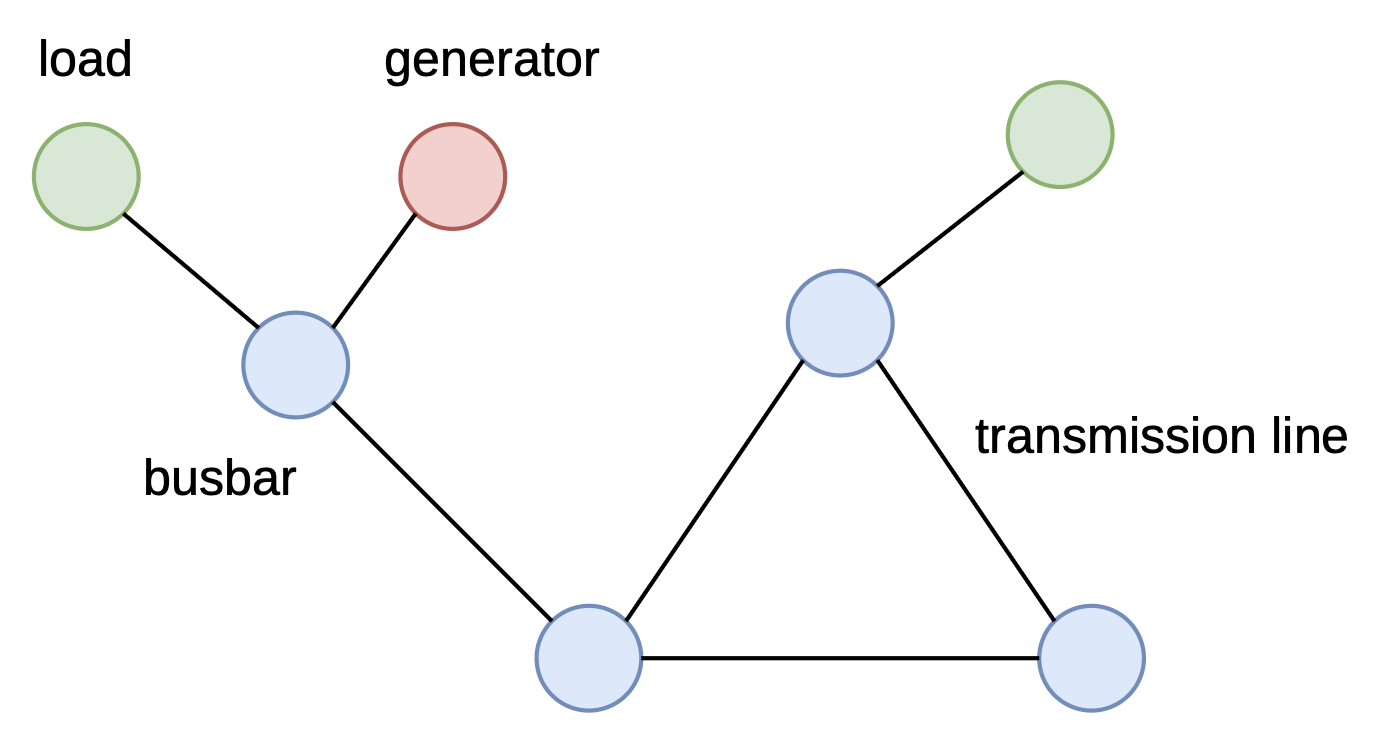
\includegraphics[width=0.92\linewidth]{figures/graph_heterogeneous_equipment.png}
  \caption{Heterogeneous equipment representation. Busbars are blue, generators
  are red, and loads are green. Physical transmission lines remain direct
  relations between busbar nodes.}
  \label{fig:heterogeneous-equipment-graph}
\end{figure}

\subsubsection{Nodes and features}
\label{subsec:heterogeneous-nodes}

For a graph with $S$ included substations, $B$ busbars per substation, $N_g$
included generators, and $N_d$ included loads, the number of nodes is
\begin{equation}
  |\mathcal{V}| = SB + N_g + N_d.
  \label{eq:heterogeneous-node-count}
\end{equation}
Busbar nodes are created exactly as in
Section~\ref{subsec:graph-busbar-nodes}. In addition, each generator and load
whose substation is present in the graph receives its own node.
\\
\\
Every busbar, generator, and load node is represented by the same ordered
eight-dimensional feature vector
\begin{equation}
  \begin{split}
  \mathbf{x}_v = [\,&
  \texttt{is\_busbar},\
  \texttt{is\_generator},\
  \texttt{is\_load},\
  \texttt{p},\
  \texttt{theta},\\
  &\texttt{time\_before\_cooldown\_sub},\
  \hl{\texttt{connected}},\
  \texttt{domain\_mask}
  \,]^{\mathsf T}\in\mathbb{R}^{8}.
  \end{split}
  \label{eq:heterogeneous-common-node-vector}
\end{equation}
The width and meaning of this vector are identical for all node
types. Table~\ref{tab:heterogeneous-node-features}
shows the value placed in every shared column. A zero in the table means that
the column is still present for that node type but is explicitly zero-filled.

\begin{table}[H]
  \centering
  \scriptsize
  \caption{Values placed in the eight feature columns shared by every node in
  the direct-line heterogeneous graph. Disconnected assets retain their node
  row but have zero power and angle.}
  \label{tab:heterogeneous-node-features}
  \setlength{\tabcolsep}{4pt}
  \begin{tabular}{L{0.34\textwidth}L{0.18\textwidth}L{0.20\textwidth}L{0.20\textwidth}}
    \toprule
    Shared feature column & Busbar node & Generator node & Load node \\
    \midrule
    \texttt{is\_busbar} & $1$ & $0$ & $0$ \\
    \texttt{is\_generator} & $0$ & $1$ & $0$ \\
    \texttt{is\_load} & $0$ & $0$ & $1$ \\
    \texttt{p} & $0$ & \texttt{gen\_p} if connected; $0$ otherwise & \texttt{load\_p} if connected; $0$ otherwise \\
    \texttt{theta} & $0$ & \texttt{gen\_theta} if connected; $0$ otherwise & \texttt{load\_theta} if connected; $0$ otherwise \\
    \texttt{time\_before\_cooldown\_sub} & Substation value & $0$ & $0$ \\
    \hl{\texttt{connected}} & $1$ & $1$ connected; $0$ disconnected & $1$ connected; $0$ disconnected \\
    \texttt{domain\_mask} & $1$ controlled; $0$ contextual & $1$ controlled; $0$ contextual & $1$ controlled; $0$ contextual \\
    \bottomrule
  \end{tabular}
\end{table}

{\color{clarif}
\paragraph{Why \texttt{connected} exists here and not in the busbar graph.}
The two disaggregated schemas give every generator and load its own node, and
that node stays in the fixed candidate graph for the whole episode whether or
not the asset is attached. When it detaches, its attachment candidates are all
masked and its measured channels are zeroed, so its row becomes
$p=0$, $\theta=0$. A generator that is attached but injecting nothing produces
the same numbers. The flag is the only channel that separates ``this asset is
not on the grid'' from ``this asset is on the grid and currently at zero''.
\\
\\
The busbar graph has no such row to disambiguate. There, a detached asset simply
stops contributing to the sum aggregated onto its busbar, and the busbar node
itself is switchgear that is never connected or disconnected. Since that schema
has a single node type, a column that would be constant for every node would
carry no information at all, whereas the disaggregated schemas share one feature
vector across all node types and a column need only be meaningful for some of
them.
\\
\\
Two consequences of that sharing are worth stating plainly. On busbar rows the
flag is written as a constant $1$ and is therefore uninformative, and on
transmission-line rows in the explicit-line schema it holds exactly the same
value as \texttt{line\_status}. The busbar graph also keeps an ambiguity the
disaggregated ones resolve: a busbar reading zero generation may have no
generator attached or an attached generator producing zero, and nothing in that
representation distinguishes the two. This is one of the information differences
between schemas discussed in Section~\ref{subsec:graph-local-global}.

\paragraph{\texttt{connected} is not the same as energized.}
The name invites a reading it does not have. \texttt{connected} is a property of
an \emph{element}, read directly from the topology vector: it says whether that
generator, load or line is currently switched onto one of its substation's
busbars. It says nothing about whether the busbar in question carries any
current. Three distinct notions are used in this work and only the last is
electrical.

\begin{table}[H]
  \centering
  \small
  \caption{Three notions that are easy to conflate. Only the last describes
  whether a node is electrically live.}
  \label{tab:connected-vs-energized}
  \setlength{\tabcolsep}{5pt}
  \begin{tabular}{L{0.20\textwidth}L{0.16\textwidth}L{0.26\textwidth}L{0.28\textwidth}}
    \toprule
    Quantity & Kind & Read from & Question it answers \\
    \midrule
    \texttt{connected} & Node feature & The element's entry in the topology
    vector & Is this element switched onto a busbar? \\
    Visibility mask & Per-node mask & Active non-structural relations reaching
    the controlled region & May this agent observe this node at all? \\
    Energized mask & Per-node mask & Incidence to at least one active
    electrical relation & Is this node electrically live? \\
    \bottomrule
  \end{tabular}
\end{table}

For a generator or load the first and the last coincide, because a detached
asset has no active attachment relation and is therefore also de-energized. For
a busbar they come apart completely: every busbar is always \texttt{connected}
by construction, while an empty busbar carries nothing. On agent~$0$ of
\texttt{bus14} under the nominal topology, all eight busbar rows read
\texttt{connected}~$=1$ while only four are energized -- the second busbar of
each substation is idle, which is precisely the busbar a splitting action would
move an element onto. The energized mask, and the readouts that use it, are
defined in Section~\ref{sec:graph-pooling}.

\paragraph{The flag is nevertheless inert in these experiments.}
The distinction it encodes is real, but the state it distinguishes never arises
here. The agents act through \texttt{change\_bus} and
\texttt{change\_line\_status}, and a change action toggles an element between
busbars without ever detaching it; separately, a substation split that isolated
a load or generator ends the episode, so no such observation is ever acted on.
In $600$ random topology actions on \texttt{bus14}, spanning $180$ episode ends,
no generator or load row was observed detached, against $150$ observed line
disconnections. Where the column does vary it duplicates something already
present: on transmission-line rows it equals \texttt{line\_status}, and on a
contextual row that loses visibility it falls to zero with the rest of that row,
which the visibility mask already reports.
\\
\\
It is therefore best read as a channel the construction supports rather than one
the reported experiments exercise. It would carry information under an action
space including \texttt{set\_bus}, which can disconnect an element, or in an
environment where assets themselves trip. Being constant, it is absorbed by the
first linear layer and costs one weight per output unit, so it is retained
rather than removed, which also keeps the input layout comparable with the runs
already completed.
}

\subsubsection{Relations and edge features}
\label{subsec:heterogeneous-relations}

% {\color{blue}Physical lines keep the busbar-to-busbar candidates of
% Equation~\ref{eq:candidate-line-edges}; what this schema adds is the asset
% attachments. For generator $g$ at substation $s(g)$, the fixed candidate graph
% contains
% \begin{equation}
%   g \rightarrow i(s(g),b)
%   \quad\text{and}\quad
%   i(s(g),b) \rightarrow g,
%   \qquad b\in\{0,\ldots,B-1\},
%   \label{eq:generator-busbar-candidates}
% \end{equation}
% that is, $B$ candidates per direction. Loads follow the same rule.
% Appendix~\ref{app:graph-construction} collects the resulting candidate-edge
% counts.}
% \\
% \\
Every candidate directed edge is represented by the same ordered feature
vector. Its physical block is
\begin{equation}
  \begin{split}
  \mathbf{p}_{uv} = [\,&
  \texttt{line\_status},\
  \texttt{rho},\
  \texttt{timestep\_overflow},\\
  &\texttt{time\_before\_cooldown\_line},\\
  &
  (\texttt{time\_next\_maintenance},\
  \texttt{duration\_next\_maintenance})_{\mathrm{optional}}
  \,]^{\mathsf T}.
  \end{split}
  \label{eq:heterogeneous-common-edge-physical-block}
\end{equation}
The two maintenance columns are appended only when scheduled maintenance is
available. The relation block is the same six-column vector for every edge:
\begin{equation}
  \begin{split}
  \mathbf{r}_{uv} = [\,&
  \texttt{relation\_physical\_line},\\
  &\texttt{relation\_same\_substation\_busbar},\\
  &\texttt{relation\_generator\_to\_busbar},\
  \texttt{relation\_busbar\_to\_generator},\\
  &\texttt{relation\_load\_to\_busbar},\
  \texttt{relation\_busbar\_to\_load}
  \,]^{\mathsf T}.
  \end{split}
  \label{eq:heterogeneous-common-edge-relation-block}
\end{equation}
The complete common edge vector is therefore
\begin{equation}
  \mathbf{e}_{uv}
  = [\,\mathbf{p}_{uv}^{\mathsf T}\mid
       \mathbf{r}_{uv}^{\mathsf T}\,]^{\mathsf T}
  \in
  \begin{cases}
    \mathbb{R}^{10}, & \text{without maintenance columns},\\
    \mathbb{R}^{12}, & \text{with maintenance columns}.
  \end{cases}
  \label{eq:heterogeneous-common-edge-vector}
\end{equation}
Its width, column order, and meaning do not change with the relation type. An
active physical-line edge fills \(\mathbf{p}_{uv}\) with its measured line
state. Every active structural or asset-attachment edge instead uses
\begin{equation}
  \mathbf{p}_{\mathrm{neutral}}
  = [\,0,1,0,0,(0,0)_{\mathrm{optional}}\,]^{\mathsf T},
  \label{eq:heterogeneous-neutral-edge-physical-block}
\end{equation}
so only the shared \texttt{rho} column is nonzero. In every active edge row,
exactly one column of \(\mathbf{r}_{uv}\) is one and the other five are zero.\\
\\
Table~\ref{tab:heterogeneous-edge-features} shows the values placed in these
common blocks for every relation.

{\color{clarif}
\paragraph{Why \texttt{rho}$=1$ on a relation that carries no current.}
The value is not a loading measurement, and it is an artifact of an encoder this
work does not report. Only the weighted GCN variant reads the \texttt{rho}
column as a scalar message weight, and for that consumer zero is the value that
\emph{deletes} a message: a structural or attachment relation weighted zero
would silently vanish from message passing. One is the multiplicative identity
that lets it pass through unscaled. The block is neutral in the sense of a
weight, not of a measurement.
\\
\\
Every result reported here uses GINE or GAT, which consume the edge vector as an
attribute through an MLP and never touch the weight path. For those encoders the
convention buys nothing, and zero -- the value already taken by every other
column of the neutral block -- would have been the consistent choice.
\\
\\
It does not destroy information. Any active physical-line edge has
\texttt{line\_status}$=1$ while the neutral block sets it to $0$; a disconnected
line's candidate edge is masked, its row zeroed and removed before message
passing, so an active row with \texttt{line\_status}$=0$ can only be structural;
and in the disaggregated schemas the relation one-hot states this explicitly.
The cost is that separating a neutral row from a loaded line becomes something
the network must learn rather than something the encoding gives it. Measured
over $6{,}000$ live-line samples on \texttt{bus14}, \texttt{rho} has mean $0.42$
and never reaches $1$ under a do-nothing policy, so the neutral value at least
sits outside the range real loadings occupy.
\\
\\
The exposure is limited and worth stating exactly. Structural relations exist
only where the schema creates them, so on agent~$0$ of \texttt{bus14} the share
of active edges carrying the neutral value is:

\begin{table}[H]
  \centering
  \small
  \caption{Active edges carrying the neutral \texttt{rho} value, agent $0$ of
  \texttt{bus14} under the nominal topology.}
  \label{tab:neutral-rho-exposure}
  \setlength{\tabcolsep}{6pt}
  \begin{tabular}{L{0.42\textwidth}L{0.30\textwidth}}
    \toprule
    Schema & Active edges affected \\
    \midrule
    Busbar, no structural augmentation & $0$ of $16$ \\
    Busbar with same-substation edges & $8$ of $24$ \\
    Disaggregated & $12$ of $28$ \\
    Disaggregated with line nodes & none; edges hold no physical block \\
    \bottomrule
  \end{tabular}
\end{table}

\noindent The candidate-action experiments are therefore untouched, as are the
busbar screens that leave the structural augmentations off. The convention is
retained rather than corrected because changing it would alter the observation
and break comparability with every completed run.
}

\begin{table}[H]
  \centering
  \scriptsize
  \caption{Values placed in the common edge-feature vector shared by every
  active directed relation in the direct-line heterogeneous graph. ``Other
  five'' refers to the remaining columns of the six-column relation block.}
  \label{tab:heterogeneous-edge-features}
  \setlength{\tabcolsep}{3pt}
  \begin{tabular}{L{0.20\textwidth}L{0.25\textwidth}L{0.17\textwidth}L{0.29\textwidth}}
    \toprule
    Directed relation & Active rule & Shared physical block & Shared relation block \\
    \midrule
    $i_o\rightarrow i_e$ and reverse (physical line) & Line online and candidate busbars match the current endpoints & Measured $\mathbf{p}_{uv}$ & \texttt{relation\_physical\_line}$=1$; other five $=0$ \\
    $i(s,b)\rightarrow i(s,b')$, $b\neq b'$ & Optional; every ordered same-substation busbar pair & $\mathbf{p}_{\mathrm{neutral}}$ & \texttt{relation\_same\_substation\_busbar}$=1$; other five $=0$ \\
    $g\rightarrow i(s(g),b)$ & Generator connected to candidate busbar $b$; direction enabled & $\mathbf{p}_{\mathrm{neutral}}$ & \texttt{relation\_generator\_to\_busbar}$=1$; other five $=0$ \\
    $i(s(g),b)\rightarrow g$ & Same mask; reverse direction enabled & $\mathbf{p}_{\mathrm{neutral}}$ & \texttt{relation\_busbar\_to\_generator}$=1$; other five $=0$ \\
    $d\rightarrow i(s(d),b)$ & Load connected to candidate busbar $b$; direction enabled & $\mathbf{p}_{\mathrm{neutral}}$ & \texttt{relation\_load\_to\_busbar}$=1$; other five $=0$ \\
    $i(s(d),b)\rightarrow d$ & Same mask; reverse direction enabled & $\mathbf{p}_{\mathrm{neutral}}$ & \texttt{relation\_busbar\_to\_load}$=1$; other five $=0$ \\
    \bottomrule
  \end{tabular}
\end{table}

\noindent Generator and load directions are selected independently as \texttt{bidirectional},
\texttt{asset\_to\_busbar}, or \texttt{busbar\_to\_asset}. The default is
\texttt{bidirectional}. Physical-line and
same-substation relations remain bidirectional.

\subsubsection{Local information boundary}

The agent-local \texttt{heterogeneous} graph contains all busbars, generators,
and loads of controlled substations. For each live boundary line it also
contains the single far-end busbar to which the line is attached, since the
line is still represented as a busbar-to-busbar edge. It never constructs a
generator or load belonging to a neighboring substation, even when that asset
is connected to the visible neighboring busbar. Neighboring private power and
angle therefore cannot enter message passing or graph readout. Inactive
far-end busbar candidates are masked in the same way as in the \texttt{bus}
schema.

{\color{clarif}
\paragraph{The consequence: a contextual busbar here carries no measurement.}
This is worth stating plainly because it is easy to read the far-end busbar as
carrying the neighbor's state, as it does in the busbar schema. It does not.
Power and angle live on asset nodes in this representation, and neighboring
assets are never constructed, so the far-end busbar row reduces to its type and
role indicators. Built on agent~$0$ of \texttt{bus14} under the nominal
topology, the two visible contextual rows are
\[
  \underbrace{[\,0,\;0,\;44.3,\;-5.51,\;0,\;0\,]}_{\texttt{bus}}
  \qquad\text{against}\qquad
  \underbrace{[\,1,\;0,\;0,\;0,\;0,\;0,\;1,\;0\,]}_{\texttt{heterogeneous}},
\]
that is $44.3$~MW of neighboring load and its angle in one schema, and exactly
zero in every measured channel in the other. The two contextual rows of the
disaggregated graph are also identical to each other, so they are not even
distinguishable as different substations.
\\
\\
Whether this is the right choice depends on which question is being asked, and
the two answers point in opposite directions.
\begin{itemize}
  \item \textbf{As an information boundary it is the defensible one.} A
  neighboring substation's generation and load are another region's private
  state. A regional operator sees the flow on the tie line, not the neighbor's
  dispatch. On that reading the busbar schema is the leaky one, and this schema
  is closer to the decentralized setting the thesis claims to model.
  \item \textbf{As a graph design it is incoherent.} Having decided to withhold
  the neighbor's power, keeping its busbar as a node buys little: it is a
  constant, anonymous, dead-end node, since edges are only created for lines
  touching the controlled domain and a contextual node therefore never connects
  to another contextual node. What the agent learns about the neighbor arrives
  through the \emph{edge} attributes of the tie line, chiefly its loading. The
  node contributes a nonlinear round trip, not new information.
\end{itemize}
The explicit-line schema resolves this by not constructing the far-end busbar at
all and placing the shared-line state on the line node instead. The three
schemas are therefore not a clean ladder of decreasing context; the
disaggregated one occupies an awkward middle position. This also makes a
\texttt{bus} against \texttt{heterogeneous} comparison something other than a
pure comparison of architectures, which is the point developed in
Section~\ref{subsec:graph-local-global}.
}


% {\color{blue}\subsubsection{Message-passing path}
% \label{subsec:heterogeneous-architecture}

% With bidirectional asset and line relations, information follows the path
% \begin{equation}
%   \text{generator}
%   \leftrightarrow
%   \text{local busbar}
%   \leftrightarrow
%   \text{remote busbar}
%   \leftrightarrow
%   \text{load}.
%   \label{eq:heterogeneous-message-path}
% \end{equation}
% One message-passing layer crosses one arrow. Generator or load information
% therefore reaches its local busbar after one layer and the adjacent remote
% busbar after two. With one-way asset relations, the reverse flow is absent.}


\subsection{Disaggregated Representation with Line Nodes}
\label{sec:heterogeneous-line-graph}

The \texttt{heterogeneous\_line} schema replaces each direct physical-line edge
with a transmission-line node between its endpoint busbars. Its node set is
\begin{equation}
  \mathcal{V} =
  \mathcal{V}_{\mathrm{bus}}
  \cup \mathcal{V}_{\mathrm{gen}}
  \cup \mathcal{V}_{\mathrm{load}}
  \cup \mathcal{V}_{\mathrm{line}}.
  \label{eq:heterogeneous-line-node-set}
\end{equation}

\begin{figure}[htbp]
  \centering
  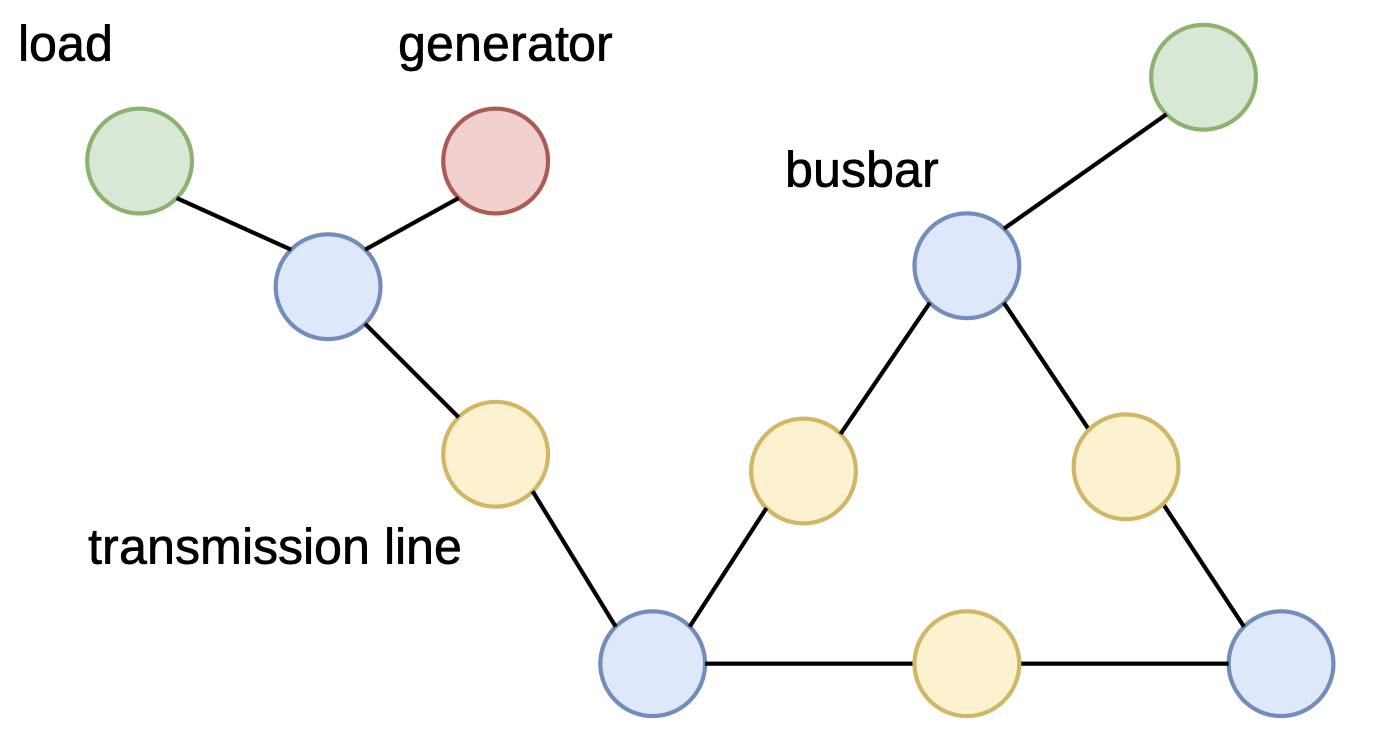
\includegraphics[width=0.92\linewidth]{figures/graph_heterogeneous_line_nodes.png}
  \caption{Heterogeneous representation with explicit transmission-line nodes.
  Yellow nodes represent physical lines and connect the blue busbars at their
  endpoints; generators and loads remain explicit terminal nodes.}
  \label{fig:heterogeneous-line-node-graph}
\end{figure}

\subsubsection{Nodes and features}
\label{subsec:heterogeneous-line-nodes}

For $S$ included substations, $B$ busbars per substation, $N_g$ generators,
$N_d$ loads, and $L$ included transmission lines, the graph contains
\begin{equation}
  |\mathcal{V}| = SB + N_g + N_d + L
  \label{eq:heterogeneous-line-node-count}
\end{equation}
nodes.
\\
\\
Every node type uses the same ordered feature vector:
\begin{equation}
  \begin{split}
  \mathbf{x}_v = [\,&
  \texttt{is\_busbar},\
  \texttt{is\_generator},\
  \texttt{is\_load},\
  \texttt{is\_transmission\_line},\\
  &\texttt{p},\
  \texttt{theta},\
  \texttt{line\_status},\
  \texttt{rho},\
  \texttt{timestep\_overflow},\\
  &\texttt{time\_before\_cooldown\_line},\\
  &(\texttt{time\_next\_maintenance},\
  \texttt{duration\_next\_maintenance})_{\mathrm{optional}},\\
  &\texttt{time\_before\_cooldown\_sub},\
  \texttt{connected},\
  \texttt{domain\_mask}
  \,]^{\mathsf T},\\
  &\mathbf{x}_v \in
  \begin{cases}
    \mathbb{R}^{13}, & \text{without maintenance columns},\\
    \mathbb{R}^{15}, & \text{with maintenance columns}.
  \end{cases}
  \end{split}
  \label{eq:heterogeneous-line-common-node-vector}
  % Placement of the optional block is explained in the note below: the vector
  % is grouped by which object owns each quantity, and maintenance is a
  % per-line quantity.
\end{equation}
{\color{clarif}
\noindent The optional block sits in the middle of the vector rather than at its
end because the ordering groups columns by the object each quantity belongs to:
type indicators, then asset measurements, then line measurements, then the
substation measurement, then the role flags. Maintenance countdowns are per-line
quantities, so appending them would place a line measurement after the
substation measurement and the role flags and split the line block in two. The
ordering is a readability convention and nothing more, since the first linear
layer is applied to the whole vector and a permutation of input columns is
absorbed by a permutation of its weight columns.
\\
\\
It has one practical cost. Appending the optional block would make the
thirteen-column layout a prefix of the fifteen-column one, so a checkpoint
trained under one setting could be loaded into the other by padding. With the
block inserted, three columns change meaning between the layouts and no such
correspondence exists. This is not hypothetical in general -- the transfer
loader already contains a routine that splices an obsolete relation column out
of an older checkpoint so that it fits the current edge vector -- but it does
not arise here, because \texttt{bus14} carries no maintenance and the transfer
study removes it from WCCI as well (Section~\ref{sec:wcci-nomaint}), leaving
both sides at thirteen columns.
}
\\
\\
The width and meaning of this vector are identical for busbar, generator, load, and
transmission-line nodes. Table~\ref{tab:heterogeneous-line-node-features}
specifies every entry; \(0\) denotes an explicitly zero-filled column, not an
omitted feature. For generators and loads, power and angle are set to zero when
the asset is disconnected.

\begin{table}[H]
  \centering
  \scriptsize
  \caption{Values placed in the common node-feature vector of the
  explicit-line heterogeneous graph, when voltage angles are carried as
  absolute per-asset values. The two maintenance rows are included only when
  maintenance observations are enabled. When the angle is instead carried as
  the drop along each line, the angle row changes owner: the generator and load
  entries become $0$ and the transmission line holds the drop across it, set to
  $0$ while the line is out (Section~\ref{sec:line-node-angle}).}
  \label{tab:heterogeneous-line-node-features}
  \setlength{\tabcolsep}{3pt}
  \begin{tabular}{L{0.30\textwidth}L{0.10\textwidth}L{0.14\textwidth}L{0.14\textwidth}L{0.20\textwidth}}
    \toprule
    Shared feature column & Busbar & Generator & Load & Transmission line \\
    \midrule
    \texttt{is\_busbar} & $1$ & $0$ & $0$ & $0$ \\
    \texttt{is\_generator} & $0$ & $1$ & $0$ & $0$ \\
    \texttt{is\_load} & $0$ & $0$ & $1$ & $0$ \\
    \texttt{is\_transmission\_line} & $0$ & $0$ & $0$ & $1$ \\
    \texttt{p} & $0$ & \texttt{gen\_p} if connected; $0$ otherwise & \texttt{load\_p} if connected; $0$ otherwise & $0$ \\
    \texttt{theta} & $0$ & \texttt{gen\_theta} if connected; $0$ otherwise & \texttt{load\_theta} if connected; $0$ otherwise & $0$ \\
    \texttt{line\_status} & $0$ & $0$ & $0$ & Observed line value \\
    \texttt{rho} & $0$ & $0$ & $0$ & Observed $\rho_\ell$ \\
    \texttt{timestep\_overflow} & $0$ & $0$ & $0$ & Observed line value \\
    \texttt{time\_before\_cooldown\_line} & $0$ & $0$ & $0$ & Observed line value \\
    \texttt{time\_next\_maintenance} & $0$ & $0$ & $0$ & Observed line value \\
    \texttt{duration\_next\_maintenance} & $0$ & $0$ & $0$ & Observed line value \\
    \texttt{time\_before\_cooldown\_sub} & Substation value & $0$ & $0$ & $0$ \\
    \texttt{connected} & $1$ & $1$ connected; $0$ disconnected & $1$ connected; $0$ disconnected & $1$ online; $0$ offline \\
    \texttt{domain\_mask} & $1$ controlled; $0$ contextual & $1$ controlled; $0$ contextual & $1$ controlled; $0$ contextual & $1$ if either endpoint is controlled; $0$ otherwise \\
    \bottomrule
  \end{tabular}
\end{table}

\subsubsection{Relations and edge features}
\label{subsec:heterogeneous-line-relations}

% {\color{blue}This schema replaces the busbar-to-busbar candidates of
% Equation~\ref{eq:candidate-line-edges} by attachments to a line node. Let
% $o(\ell)$ and $e(\ell)$ denote the origin and extremity substations of line
% $\ell$. For every busbar index $b$, the fixed candidate graph contains
% \begin{equation}
%   \begin{aligned}
%     i(o(\ell),b) &\rightarrow \ell, &\qquad \ell &\rightarrow i(o(\ell),b), \\
%     i(e(\ell),b) &\rightarrow \ell, &\qquad \ell &\rightarrow i(e(\ell),b),
%   \end{aligned}
%   \qquad b\in\{0,\ldots,B-1\},
%   \label{eq:heterogeneous-line-candidates}
% \end{equation}
% that is, $2B$ candidates per end.}
% \\
% \\
% The line direction is \texttt{bidirectional}, \texttt{line\_to\_busbar}, or
% \texttt{busbar\_to\_line}; a one-way mode retains only one column of
% Equation~\ref{eq:heterogeneous-line-candidates}. An online line therefore has
% four active attachments in the bidirectional case and two in a one-way case.
% \\
% \\
Every candidate directed edge uses the same ordered nine-dimensional feature
vector:
\begin{equation}
  \begin{split}
  \mathbf{e}_{uv} = [\,&
  \texttt{relation\_same\_substation\_busbar},\\
  &\texttt{relation\_busbar\_to\_line\_origin},\
  \texttt{relation\_line\_origin\_to\_busbar},\\
  &\texttt{relation\_busbar\_to\_line\_extremity},\
  \texttt{relation\_line\_extremity\_to\_busbar},\\
  &\texttt{relation\_generator\_to\_busbar},\
  \texttt{relation\_busbar\_to\_generator},\\
  &\texttt{relation\_load\_to\_busbar},\
  \texttt{relation\_busbar\_to\_load}
  \,]^{\mathsf T}\in\mathbb{R}^{9}.
  \end{split}
  \label{eq:heterogeneous-line-common-edge-vector}
\end{equation}
These edges contain no continuous line-state attributes because the
transmission-line node already contains \texttt{rho}, status, overflow,
cooldown, and maintenance. For an active edge, exactly one relation column is
one and the other eight are zero. An inactive candidate has all nine entries set
to zero and is removed by \texttt{edge\_mask}$=0$ before message passing.
Table~\ref{tab:heterogeneous-line-edge-features} gives the active rule and the
nonzero entries for every relation.

\begin{table}[H]
  \centering
  \scriptsize
  \caption{Nonzero entries in the common 9-column edge-feature vector of the
  explicit-line heterogeneous graph. All relation columns not named in a row
  are zero.}
  \label{tab:heterogeneous-line-edge-features}
  \setlength{\tabcolsep}{3pt}
  \begin{tabular}{L{0.20\textwidth}L{0.31\textwidth}L{0.38\textwidth}}
    \toprule
    Directed relation & Active rule & Relation column set to $1$ \\
    \midrule
    $i(s,b)\rightarrow i(s,b')$, $b\neq b'$ & Optional; every ordered same-substation pair & \texttt{relation\_same\_substation\_busbar} \\
    $i_o\rightarrow\ell$ & Online line, current origin busbar, direction enabled & \texttt{relation\_busbar\_to\_line\_origin} \\
    $\ell\rightarrow i_o$ & Same mask; reverse direction enabled & \texttt{relation\_line\_origin\_to\_busbar} \\
    $i_e\rightarrow\ell$ & Online line, current extremity busbar, direction enabled & \texttt{relation\_busbar\_to\_line\_extremity} \\
    $\ell\rightarrow i_e$ & Same mask; reverse direction enabled & \texttt{relation\_line\_extremity\_to\_busbar} \\
    $g\rightarrow i(s(g),b)$ & Generator attached to $b$; direction enabled & \texttt{relation\_generator\_to\_busbar} \\
    $i(s(g),b)\rightarrow g$ & Same mask; reverse direction enabled & \texttt{relation\_busbar\_to\_generator} \\
    $d\rightarrow i(s(d),b)$ & Load attached to $b$; direction enabled & \texttt{relation\_load\_to\_busbar} \\
    $i(s(d),b)\rightarrow d$ & Same mask; reverse direction enabled & \texttt{relation\_busbar\_to\_load} \\
    \bottomrule
  \end{tabular}
\end{table}

\subsubsection{Local information boundary}

In the agent-local \texttt{heterogeneous\_line} graph, every line touching a
controlled substation is itself part of the agent's observation/action graph.
Only controlled busbars, generators, loads, and the corresponding line nodes
are constructed. A boundary line node is connected only to its endpoint
busbar inside the controlled domain; no candidate edge to its non-controlled
endpoint and no neighboring busbar, generator, or load node is created. The
line node already carries the shared measurements, so no far-end context is
needed. If the line is disconnected, the line node remains visible with
\texttt{line\_status}$=0$, but all of its busbar-attachment edges are inactive.
This construction is unchanged by the neighbor-inclusion option.

% \noindent Origin, extremity, and direction have separate relation types. Generator and
% load attachments follow Equation~\ref{eq:generator-busbar-candidates};
% same-substation relations remain optional.

% \subsubsection{Message-passing path}
% \label{subsec:heterogeneous-line-message-path}

% The direct-line graph connects endpoint busbars in one hop. The explicit-line
% graph uses
% \begin{equation}
%   i_o \rightarrow \ell \rightarrow i_e,
%   \label{eq:heterogeneous-line-two-hop-path}
% \end{equation}
% so endpoint exchange requires two layers. The first layer forms
% \begin{equation}
%   \mathbf{h}_{\ell}^{(1)}
%   = f_{\ell}\!\left(
%       \mathbf{h}_{\ell}^{(0)},
%       \mathbf{h}_{i_o}^{(0)},
%       \mathbf{h}_{i_e}^{(0)}
%     \right),
% \end{equation}
% and the second returns this joint state to the endpoints. Later layers enlarge
% the receptive field. The edges around the line node are bidirectional: the line gathers both endpoints and sends the updated state back; endpoint exchange is possible.

\subsection{Local actor information boundary and the global state graph}
\label{subsec:graph-local-global}

Each agent $a$ controls a set of substations $\mathcal{C}_a$. A
boundary line connects $\mathcal{C}_a$ to another agent's domain, and
its far-end busbar is the only possible neighboring busbar. The local graph
exposes only the boundary information required by its representation.

{\color{clarif}
\paragraph{Why one hop, and why not more.}
The one-hop cut is a modelling decision and it is worth separating from two
arguments that do not support it. The first is that an agent cannot act on a
neighboring substation, so it need not observe one. Controllability and
observability are independent: a regional control room does not operate its
neighbor's substations but does observe them, through state estimation on an
extended model, tie-line telemetry, and inter-operator data exchange. On
realism alone, the local graphs used here are more restrictive than a real
control room, not less.
\\
\\
The second is that one hop is the natural amount of exterior to keep. Power flow
has no one-hop boundary. The established treatment in power systems is an
external network equivalent, which reduces everything outside the area to a
small model preserving \emph{boundary} behaviour, and which deliberately
discards the neighbor's internal dispatch while retaining the boundary
injections and the stiffness seen from the boundary. Read that way, the
neighbor's own generation and load is the least useful part of the exterior: it
is a single bus of an unbounded remainder. What determines whether a switching
action is safe inside $\mathcal{C}_a$ is the post-action flow there, and the
exterior enters that calculation only through the boundary condition -- the
loading of the tie line and the angle across it, both of which the schemas
already carry on the line itself
(Section~\ref{sec:line-node-angle}).
\\
\\
The argument that does support keeping the actor local is not physical but
methodological. An actor that observes everything is a centralized controller
with extra steps, and the question this thesis asks is how far a policy
conditioned on a regional view can go. The centralized critic already reads the
global state, so the value estimate is not blind; only the policy is. That
compensates in part, but not completely: where the optimal action depends on
exterior state the actor cannot see, the policy can only learn an average over
it, which is the standard limitation of a decentralized partially observed
setting and is exactly the regime in which a remote contingency decides whether
a local action was correct.
\\
\\
The honest position is therefore that context depth is an ablation rather than a
justified constant, and it is treated as one: \texttt{gnn\_include\_neighbors}
switches it, and the two settings are compared under otherwise identical
configurations.

\paragraph{In what sense the earlier construction was defective.}
Since observing a neighbor is not in itself improper, it is worth being precise
about what was wrong with the construction this section replaces, because it was
not simply that it revealed more.
\\
\\
The earlier rule expanded every substation of the region into all of its
busbars and marked them permanently valid. In effect an agent could see anything
that shared a substation label with something it touched. That is a convention
of the data model, not an electrical relation: two busbars of one substation are
separate electrical nodes whenever the substation is split. Built on agent~$0$
of \texttt{bus14}, with contextual substation~$3$ split so that its $44.3$~MW
load sits on the second busbar while the agent's lines attach to the first, the
earlier construction placed that load in the observation on a node with
\emph{no active edge at all}. Electrically it was as remote from the agent as any
other bus in the grid.
\\
\\
Two things follow, and the second matters more than the first. Such a node is
isolated, so it receives and sends no messages: the value never entered message
passing and instead contributed its raw feature row directly to the mean
readout. The information was therefore not usable context but an unstructured
additive term in the pooled vector. And because the split is an action of the
\emph{neighboring} agent, that agent's decisions moved quantities inside this
agent's observation without any change in this agent's electrical situation,
adding an observation-level non-stationarity on top of the one decentralized
training already has.
\\
\\
The correction is therefore about the criterion and the delivery path rather
than about volume. Requiring a live electrical connection replaces a naming
convention with a physical one, and removes rows that the graph could not
process in any case. It does not follow that the resulting boundary is the
correct amount of exterior; as argued above, it is a conservative one, and an
explicit exterior equivalent would be the principled alternative.
}

\subsubsection{Visibility and masking}

Candidate rows are retained for fixed tensor shapes, but a contextual busbar
is visible only while a live boundary line connects it to the controlled
region. Otherwise its entire feature row is zeroed, every incident edge is
deactivated and removed before message passing, and the row is excluded from
pooling---including the denominator of a mean. It therefore affects neither
message passing nor the readout. Same-substation edges cannot restore
visibility.
\\
\\
Controlled nodes remain visible when disconnected. In
\texttt{heterogeneous\_line}, a shared-line node also remains visible because
it belongs to the agent graph, although its attachment edges are inactive when
the line is offline. Physical and attachment relations are active only when
the line is online and the current busbar assignments match their candidate
endpoints. Neighboring generators and loads are never constructed, and the
explicit-line representation creates no far-end attachment. Pooling is thus a
summary operation, not the information-security boundary.

\subsubsection{Representation-dependent information}

The representations are not information-equivalent. The busbar schema exposes
the most neighboring information because it aggregates assets at the far-end
busbar; the heterogeneous schema exposes only that busbar; and the
explicit-line schema exposes only the shared line.

\begin{table}[H]
  \centering
  \small
  \caption{Information from another agent's domain visible to a local actor.}
  \label{tab:local-information-boundary}
  \setlength{\tabcolsep}{4pt}
  \begin{tabular}{L{0.24\textwidth}L{0.64\textwidth}}
    \toprule
    Representation & Neighbor information available \\
    \midrule
    \texttt{bus} & Shared-line edge and attached far-end busbar, including aggregated generator/load power and angles \\
    \texttt{heterogeneous} & Shared-line edge and attached far-end busbar; no neighboring generator/load nodes or private-asset state \\
    \texttt{heterogeneous\_line} & Shared-line node only; no neighboring busbar, equipment, or far-end attachment \\
    \bottomrule
  \end{tabular}
\end{table}

Comparing these representations therefore compares both architectures and
actor information sets.

\subsubsection{Legacy compatibility and centralized state}

{\color{red}
The legacy construction kept all neighboring busbars, and in heterogeneous
graphs their private assets, visible even without a live boundary connection.
Such rows could enter pooling even when isolated from message passing.
Setting \texttt{gnn\_context\_requires\_connection=false} restores this legacy
visibility for A/B tests; legacy and leakage-free checkpoints are therefore
not strictly comparable.}
\\
\\
This boundaries apply only to decentralized actor graphs. The centralized
critic still uses the full-grid state graph during training, while
execution uses each actor's local graph, as required by MAPPO's centralized-
training, decentralized-execution setup~\cite{yu2022mappo}.

\subsection{Graph actor and centralized critic}
\label{subsec:graph-representation-encoder-boundary}

\begin{figure}[H]
  \color{black}
  \centering
  \resizebox{\textwidth}{!}{%
    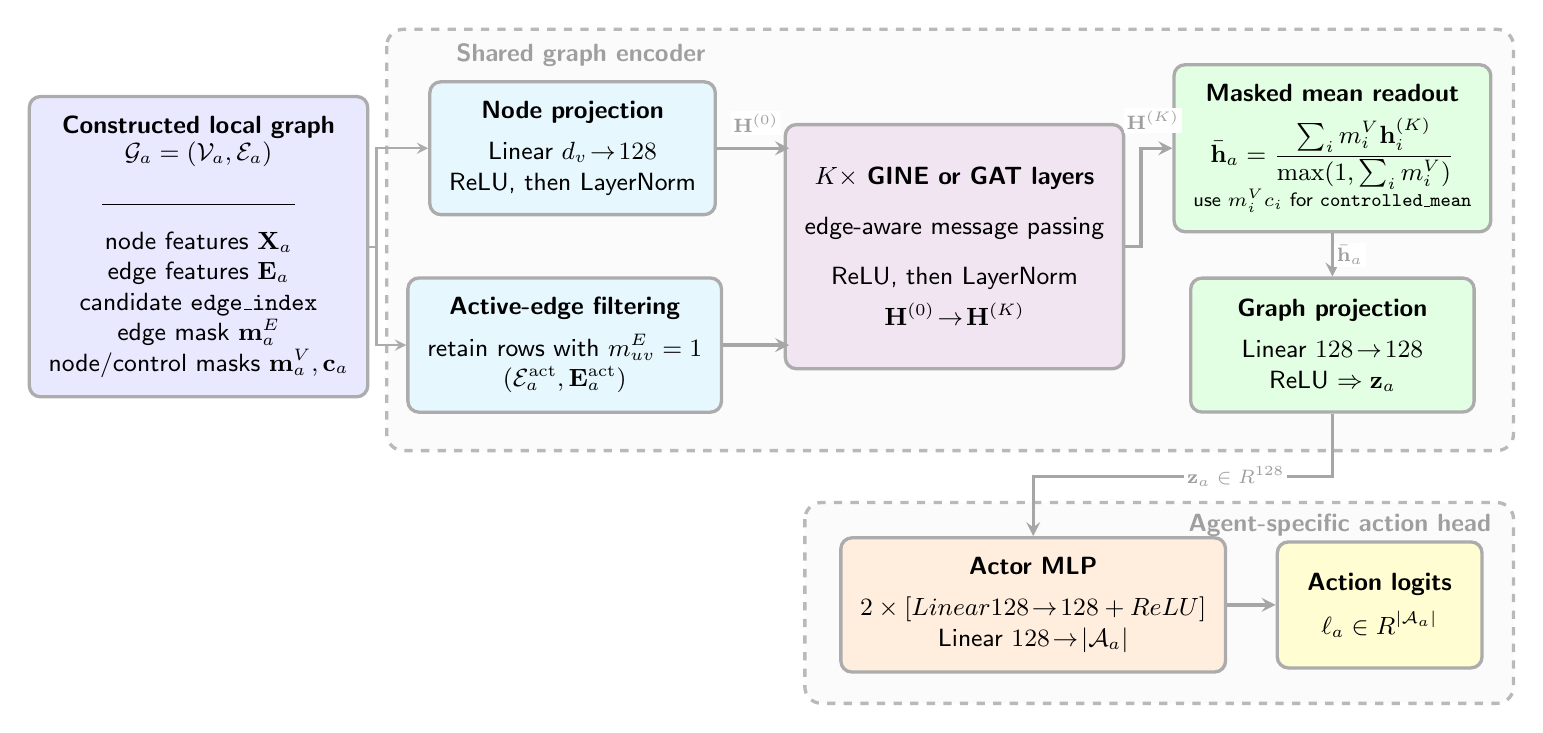
\begin{tikzpicture}[
  >=stealth,
  font=\small\sffamily,
  flow/.style={->, very thick, draw=gray!70},
  branch/.style={->, thick, draw=gray!65},
  stage/.style={
    draw=gray!65,
    very thick,
    rounded corners=4pt,
    align=center,
    text=black,
    inner sep=7pt
  },
  note/.style={font=\scriptsize\sffamily, text=gray!75, fill=white, inner sep=1pt},
  lane/.style={
    draw=gray!55,
    dashed,
    rounded corners=6pt,
    fill=gray!3,
    very thick
  }
]

% Draw.io-style group containers.
\path[lane] (1.64,2.76) rectangle (15.95,-2.59);
\node[anchor=west, font=\bfseries\small\sffamily, text=gray!75]
  at (2.40,2.43) {Shared graph encoder};

\path[lane] (6.95,-3.25) rectangle (15.95,-5.80);
\node[anchor=west, font=\bfseries\small\sffamily, text=gray!75]
  at (11.7,-3.54) {Agent-specific action head};

% Constructed graph.
\node[
  stage,
  fill=blue!9,
  minimum width=3.40cm,
  minimum height=3.45cm
] (graph) at (-0.75,0) {
  {\bfseries Constructed local graph}\\[-1pt]
  $\mathcal{G}_a=(\mathcal{V}_a,\mathcal{E}_a)$\\[5pt]
  \rule{2.45cm}{0.35pt}\\[5pt]
  node features $\mathbf{X}_a$\\
  edge features $\mathbf{E}_a$\\
  candidate \texttt{edge\_index}\\
  edge mask $\mathbf{m}^{E}_a$\\
  node/control masks $\mathbf{m}^{V}_a,\mathbf{c}_a$
};

% Encoder inputs.
\node[
  stage,
  fill=cyan!10,
  minimum width=3.10cm,
  minimum height=1.65cm
] (nodeproj) at (4,1.25) {
  {\bfseries Node projection}\\[4pt]
  Linear $d_v\!\rightarrow\!128$\\
  ReLU, then LayerNorm
};

\node[
  stage,
  fill=cyan!10,
  minimum width=3.10cm,
  minimum height=1.65cm
] (filter) at (3.9,-1.25) {
  {\bfseries Active-edge filtering}\\[4pt]
  retain rows with $m^E_{uv}=1$\\
  $(\mathcal{E}^{\mathrm{act}}_a,\mathbf{E}^{\mathrm{act}}_a)$
};

% Repeated message-passing block.
\node[
  stage,
  fill=violet!10,
  minimum width=4.20cm,
  minimum height=3.10cm
] (message) at (8.85,0) {
  {\bfseries $K\times$ GINE or GAT layers}\\[7pt]
  edge-aware message passing\\[7pt]
  ReLU, then LayerNorm\\[4pt]
  $\mathbf{H}^{(0)}\!\rightarrow\!\mathbf{H}^{(K)}$
};

% Readout and shared graph projection.
\node[
  stage,
  fill=green!11,
  minimum width=3.60cm,
  minimum height=1.70cm
] (pool) at (13.65,1.25) {
  {\bfseries Masked mean readout}\\[5pt]
  $\displaystyle
    \bar{\mathbf h}_a=
    \frac{\sum_i m^V_i\mathbf h_i^{(K)}}
         {\max(1,\sum_i m^V_i)}$\\[-1pt]
  {\scriptsize use $m^V_i c_i$ for \texttt{controlled\_mean}}
};

\node[
  stage,
  fill=green!11,
  minimum width=3.60cm,
  minimum height=1.70cm
] (graphproj) at (13.65,-1.25) {
  {\bfseries Graph projection}\\[4pt]
  Linear $128\!\rightarrow\!128$\\
  ReLU $\Rightarrow \mathbf z_a$
};

% Per-agent policy head and logits.
\node[
  stage,
  fill=orange!13,
  minimum width=4.80cm,
  minimum height=1.60cm
] (actor) at (9.85,-4.55) {
  {\bfseries Actor MLP}\\[4pt]
  $2\times[\text{Linear }128\!\rightarrow\!128+\text{ReLU}]$\\
  Linear $128\!\rightarrow\!|\mathcal A_a|$
};

\node[
  stage,
  fill=yellow!18,
  minimum width=2.60cm,
  minimum height=1.60cm
] (logits) at (14.25,-4.55) {
  {\bfseries Action logits}\\[5pt]
  $\boldsymbol{\ell}_a\in
   \mathbb{R}^{|\mathcal A_a|}$
};

% Data flow.
\draw[branch] (graph.east) -- (1.51,0) |- (nodeproj.west);
\draw[branch] (graph.east) -- (1.51,0) |- (filter.west);
\draw[flow] (nodeproj.east) -- node[note, above=4pt, pos=0.54] {$\mathbf H^{(0)}$} (6.75,1.25);
\draw[flow] (filter.east) -- (6.75,-1.25);
\draw[flow] (message.east) -- (11.22,0) |- node[note, above=5pt, pos=0.69] {$\mathbf H^{(K)}$} (pool.west);
\draw[flow] (pool.south) -- node[note, right] {$\bar{\mathbf h}_a$} (graphproj.north);
\draw[flow] (graphproj.south) -- (13.65,-2.92) -| node[note, near start, right] {$\mathbf z_a\in\mathbb R^{128}$} (actor.north);
\draw[flow] (actor.east) -- (logits.west);

\end{tikzpicture}
%
  }
  \caption{End-to-end graph-actor architecture. Candidate edges masked by the
  current topology are removed before message passing. The graph encoder and
  its output projection are shared across agents, whereas the final MLP has one
  output per action available to agent $a$ and is therefore agent-specific.}
  \label{fig:graph-actor-pipeline}
\end{figure}

GINE and GAT use the same actor pipeline and differ only in the
message-passing operator. In the reported configuration, the input node
projection and the two message-passing layers have 128 features. LayerNorm is
applied after the input projection and after each message-passing layer. The
graph readout produces a 128-dimensional embedding, followed by an
agent-specific action head with two 128-unit hidden layers. The graph encoder
and output projection are shared across agents, whereas the action heads are
separate because their action-set sizes may differ.
\\
\\
This is the default configuration. The
candidate-scoring alternative of Section~\ref{sec:candidate-action-scoring}
replaces this head.
\\
\\
The centralized critic is a separate MLP over the normalized flat state. It
does not reuse the actor graph embedding and is used only during centralized
training. Its flat-state normalization is independent of the graph-input
normalization. The exact GINE and GAT updates, graph readout, output projection,
and action-head equations are given in
Appendix~\ref{app:gine-architecture}.

\begin{tcolorbox}[
  colframe=red!75!black,
  colback=red!5!white,
  title=Chapter Summary (1/3): Graph Construction and Model
]
\textbf{Purpose:} Define how the electrical state becomes the input of each
actor and how that input is encoded.

\begin{itemize}
  \item \textbf{Input processing:} Continuous physical quantities can be
  divided by fixed physical scales and optionally standardized from training
  statistics. The loading ratio \texttt{rho}, binary features, and masks remain
  unchanged. The graph-screening experiments use raw features; the cross-grid
  transfer study uses deterministic physical scaling.
  \item \textbf{Dynamic topology:} Nodes and candidate edges remain fixed, while
  time-dependent edge and node masks retain only the relations and contextual
  nodes that are electrically connected to the controlled region. An inactive
  contextual candidate has a zero feature row and participates in neither
  message passing nor readout.
  \item \textbf{Graph representations:} The \texttt{bus} schema aggregates
  equipment on busbars; \texttt{heterogeneous} gives generators and loads their
  own nodes; and \texttt{heterogeneous\_line} also represents each transmission
  line as a node. This changes both the feature location and the number of
  message-passing steps between physical objects.
  \item \textbf{Actor and critic:} Each actor receives its controlled region and
  only the schema-specific boundary context of
  Table~\ref{tab:local-information-boundary}. The reference architecture uses a two-layer,
  128-feature GINE or GAT encoder shared across agents, followed by an
  agent-specific action head. The centralized critic remains a separate MLP
  over the normalized full-grid flat state.
\end{itemize}

\textbf{Takeaway:} The graph variants change both how state is represented and
how much neighboring information is available. The MAPPO training structure
and agent partition remain unchanged, but the three representations must not be
described as information-equivalent.
\end{tcolorbox}

\section{Substation Representation: Direct Edges and Summary Nodes}
\label{sec:substation-representation}

Two optional factors change how information is exchanged inside a substation.
The factor $e$ adds direct same-substation busbar edges. The factor $n$ adds one
learned substation-summary node per included substation. Both augmentations are
part of the constructed graph $G_a$ shown at the left of
Figure~\ref{fig:graph-actor-pipeline}; their nodes and edges therefore enter the
same node projection, edge filtering, and message-passing pipeline as the base
graph.

\subsection{Direct same-substation edges (e)}
\label{subsec:graph-relation-edges}

In addition to physical-line relations, the augmentation inserts
$i(s,b)\rightarrow i(s,b')$ for every ordered pair $b\neq b'$ of busbars in the
same included substation. The edges are therefore bidirectional between each
pair of busbars, remain active throughout the episode, and do not represent an
electrical connection. Figure~\ref{fig:same-substation-busbar-edge} shows this
relation for the busbar and disaggregated schemas.
\\
\\
Table~\ref{tab:same-substation-augmentation-features} gives the exact feature
values of the added edges. The neutral value \texttt{rho}$=1$ is used whenever
the schema contains physical edge attributes; every other physical attribute is
zero.

{\color{clarif}
\paragraph{These edges are added inside neighboring substations too.}
The augmentation runs over every substation of the region, contextual ones
included, so a neighboring substation's busbars are joined to each other exactly
as controlled ones are. That interacts with the information boundary of
Section~\ref{subsec:graph-local-global} in a way worth making explicit.
\\
\\
A same-substation relation does \emph{not} carry visibility. Grid2Op has no bus
coupler: busbar assignment is the topology, and two busbars of one substation
are separate electrical nodes. The relation is a computational device encoding
that an element can be moved between them, which is a statement about an action
space rather than about conductivity -- and, for a contextual substation, about
\emph{another} agent's action space. The visibility rule therefore excludes it,
together with self relations, when deciding whether a contextual node is
connected to the controlled region.
\\
\\
The effect is measurable. Take agent~$0$ of \texttt{bus14} with contextual
substation~$3$ split so that its $44.3$~MW load sits on the busbar the agent's
lines do \emph{not} attach to:

\begin{table}[H]
  \centering
  \small
  \caption{Status of the contextual busbar carrying $44.3$~MW, under the two
  constructions and the two settings of this augmentation.}
  \label{tab:same-substation-visibility}
  \setlength{\tabcolsep}{6pt}
  \begin{tabular}{llccc}
    \toprule
    Construction & Same-substation edges & Visible & Active degree & Load seen \\
    \midrule
    Earlier & off & yes & $0$ & $44.3$ \\
    Earlier & on  & yes & $2$ & $44.3$ \\
    Current & off & no  & $0$ & $0$ \\
    Current & on  & no  & $0$ & $0$ \\
    \bottomrule
  \end{tabular}
\end{table}

\noindent The second row is the important one. Under the earlier construction this
augmentation upgraded the leak: without it the unreachable busbar was an
isolated node contributing only to the readout, whereas with it the busbar
became connected to its sibling and its load propagated into the agent's own
region through message passing. The cells of Screen~C that enable this factor
are therefore the most affected by the construction they were run under. Under
the current rule the node is invisible and its structural edges are inactive in
both settings, so the augmentation changes message passing only among nodes the
agent is entitled to see.

\paragraph{Being entitled to see two nodes is not a reason to relate them.}
One case survives the correction. When a contextual substation is split so that
both of its busbars are attached to the agent by live lines, both are visible
and the same-substation relation between them is active: on agent~$0$ of
\texttt{bus14} with substation~$3$ split in this way, the pair of directed edges
between its two busbars carries messages. This is not a boundary violation,
since each endpoint is legitimately observable, but it is questionable on two
other grounds.
\\
\\
The relation asserts that an element can be moved between the two busbars. That
is a statement about an action space, and for a contextual substation it is a
statement about \emph{another agent's} action space, which this agent can
neither exercise nor anticipate. The same reasoning already excludes structural
relations from carrying visibility, so allowing them to carry messages between
two contextual nodes is inconsistent with a decision already taken elsewhere in
the construction.
\\
\\
The physical objection is stronger. Two busbars of one substation are separate
electrical nodes, and the relation is justified inside the controlled domain
only because the agent can join them by acting. Between two contextual busbars
it is neither electrical nor reachable by any action available here, and it
creates a message path that crosses the boundary twice: information leaving the
agent on one line can return on another through a coupling that does not exist,
where the true path runs through the agent's own internal topology.
\\
\\
Both structural augmentations are therefore restricted to controlled
substations. The fixed candidate shape does not prevent this, since the
controlled substations are themselves a static set, and it also separates a
factor that would otherwise be confounded: enabling the augmentation now changes
relations inside the controlled domain only, rather than changing them there and
between contextual nodes at the same time. On agent~$0$ of \texttt{bus14} with
substation~$3$ split as above, the number of active same-substation edges falls
from ten to eight, and the two that related the neighbor's busbars to each other
are gone.
}

\begin{table}[H]
  \centering
  \small
  \caption{Node and edge features introduced by the direct same-substation
  augmentation. ``None'' means that the augmentation neither adds nodes nor
  changes the features of existing nodes.}
  \label{tab:same-substation-augmentation-features}
  \setlength{\tabcolsep}{4pt}
  \begin{tabular}{L{0.20\textwidth}L{0.16\textwidth}L{0.54\textwidth}}
    \toprule
    Graph schema & Added node features & Feature values on each added directed edge \\
    \midrule
    Busbar & None & \texttt{rho}$=1$; all other physical-line features are $0$. \\
    Disaggregated & None & \texttt{rho}$=1$ and \texttt{relation\_same\_substation\_busbar}$=1$; all other entries are $0$. \\
    Disaggregated with line nodes & None & \texttt{relation\_same\_substation\_busbar}$=1$; the other eight relation entries are $0$. \\
    \bottomrule
  \end{tabular}
\end{table}

\begin{figure}[htbp]
  \centering
  \begin{subfigure}[b]{0.49\linewidth}
    \centering
    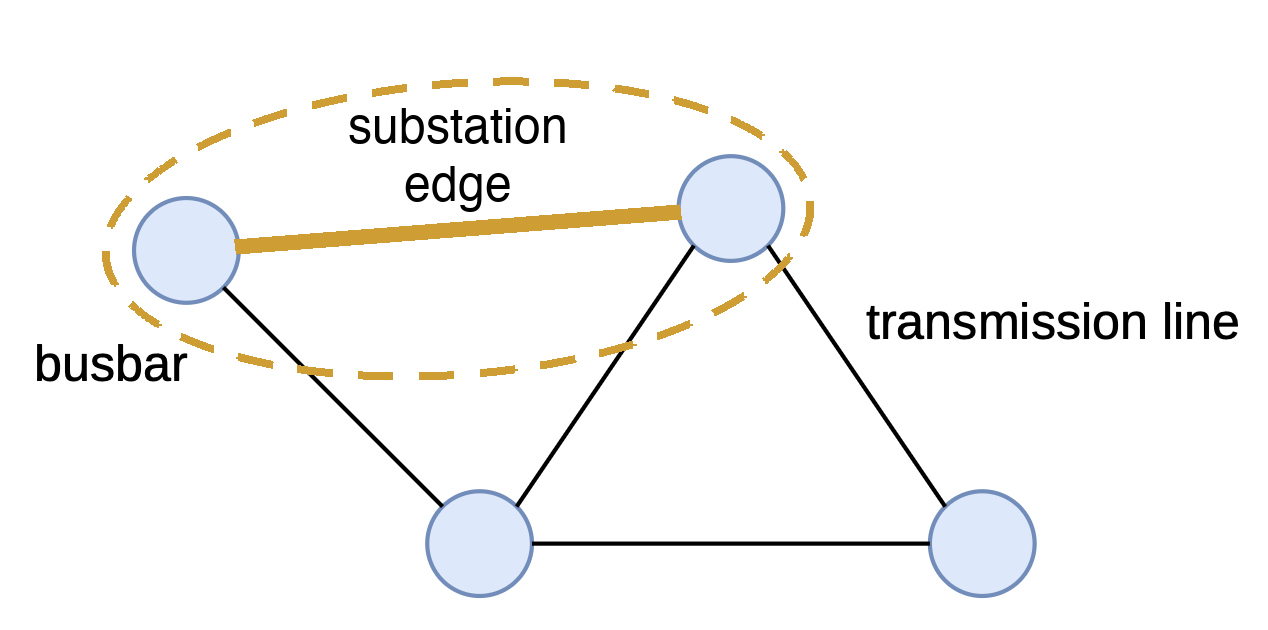
\includegraphics[width=\linewidth]{figures/graph_same_substation_edge_bus.png}
    \caption{Busbar graph.}
    \label{fig:same-substation-edge-bus}
  \end{subfigure}
  \hfill
  \begin{subfigure}[b]{0.49\linewidth}
    \centering
    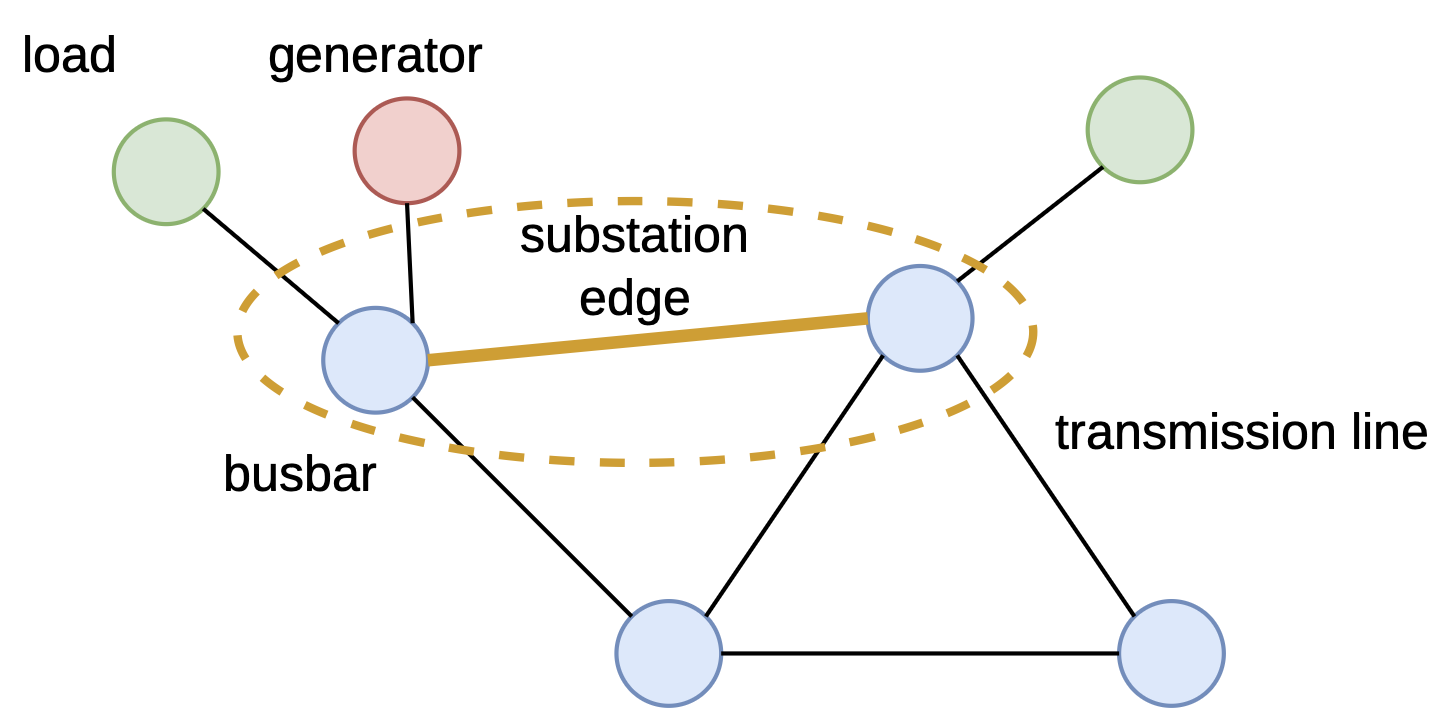
\includegraphics[width=\linewidth]{figures/graph_same_substation_edge.png}
    \caption{Disaggregated graph.}
    \label{fig:same-substation-edge-hetero}
  \end{subfigure}
  \caption{Direct same-substation busbar relation, shown in the two schemas of
  Section~\ref{sec:graph-representation}. The highlighted orange edge allows two
  busbars belonging to the same substation to exchange messages; it is a
  computational relation and not a physical transmission line. In~(a) the
  generator and load quantities are aggregated into the busbar features, whereas
  in~(b) they are separate nodes. The relation is identical in both cases: it
  connects two busbars of one substation and does not depend on the node types
  attached to them.}
  \label{fig:same-substation-busbar-edge}
\end{figure}


\subsection{Substation summary nodes (n)}
\label{sec:substation-summary-nodes}

In all experiments, augmentation $n$ adds one learned summary node $u_s$ for
each included substation $s$ and connects it in both directions to every busbar
in $\mathcal{B}(s)$:
\begin{equation}
  \mathcal{E}_{\mathrm{sub}} =
  \left\{
    (i,u_s),(u_s,i)
    \;\middle|\;
    i\in\mathcal{B}(s)
  \right\};
  \label{eq:substation-node-edges}
\end{equation}
For $S$ included substations with $B$ busbars each, this adds $S$ nodes and
$2SB$ directed edges. Each $u_s$ gathers information from its busbars and sends
the result back, so two busbars in the same substation communicate in two steps:
$i(s,b)\rightarrow u_s\rightarrow i(s,b')$. It therefore provides the same
intra-substation communication role as the direct relation in
Figure~\ref{fig:same-substation-busbar-edge}. Only busbars connect directly to
$u_s$; other node types reach it through their busbar attachments.
Figure~\ref{fig:substation-summary-node} shows this construction.

{\color{clarif}
\paragraph{Summary nodes exist only for controlled substations.}
The augmentation is restricted to the agent's own substations, for the reason
given in Section~\ref{subsec:graph-relation-edges}: a summary node relates every
busbar it gathers, and outside the controlled domain that relation is one the
agent can neither act on nor make sense of. Without the restriction a
neighboring substation would receive a summary node as well, and two of its
busbars could exchange through it even with the direct relation removed, so both
augmentations have to be restricted together for either restriction to mean
anything.
\\
\\
The earlier behaviour was also close to inert. On agent~$0$ of \texttt{bus14}
under the nominal topology, each controlled substation's summary node gathers
both of its busbars, whereas a contextual one gathered exactly one. Summarizing
a single node is an identity up to the learned transform: the round trip
$i(s,b)\rightarrow u_s\rightarrow i(s,b)$ returns to its origin while consuming
two message-passing steps, the entire depth at the two-layer setting used
throughout, and adds a learned constant row to an ordinary mean readout.
\\
\\
Two consequences are worth recording. Summary nodes are appended by the encoder
after visibility has been decided, and they gather only busbars that are both
controlled and currently visible, so no contextual state reaches the agent by
this route under either setting. And because the virtual-node readout attaches
to summary nodes where they exist, contextual busbars no longer reach the graph
summary directly; they influence it through the controlled busbars they are
connected to, consistent with reading the graph embedding as a description of
the region the agent controls.
}
\\
\begin{figure}[htbp]
  \centering
  \begin{subfigure}[b]{0.49\linewidth}
    \centering
    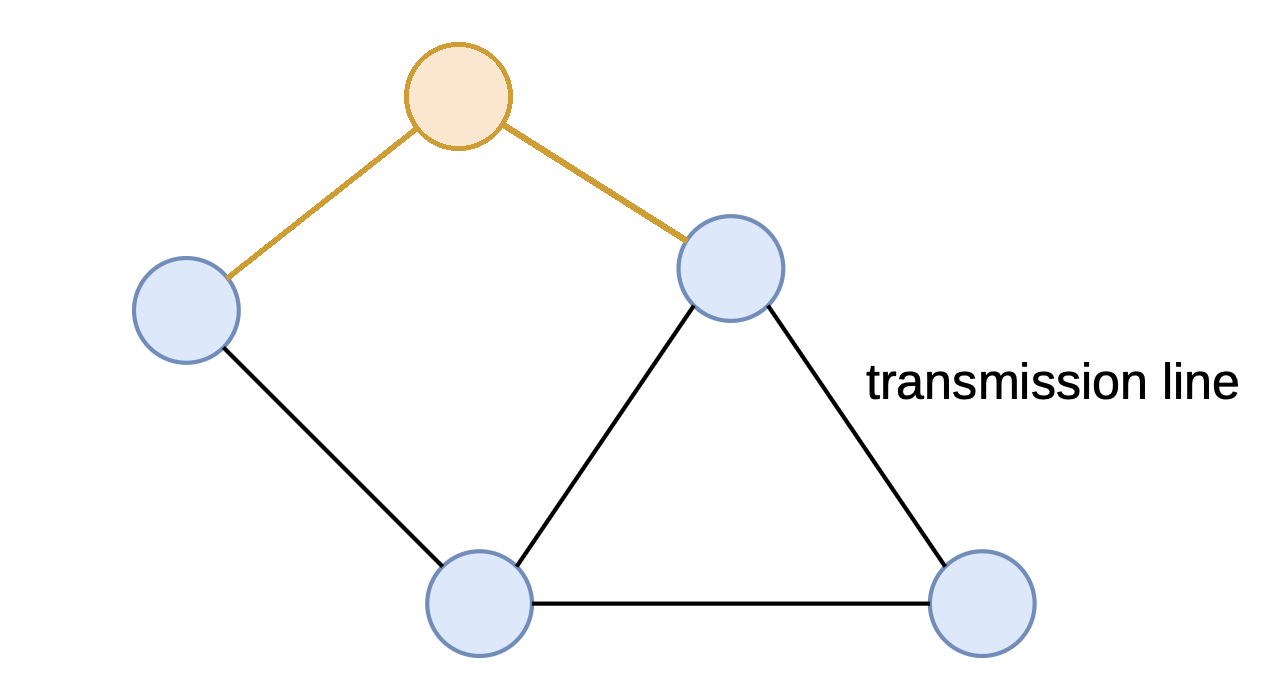
\includegraphics[width=\linewidth]{figures/graph_substation_summary_node_bus.png}
    \caption{Busbar graph.}
    \label{fig:substation-summary-node-bus}
  \end{subfigure}
  \hfill
  \begin{subfigure}[b]{0.49\linewidth}
    \centering
    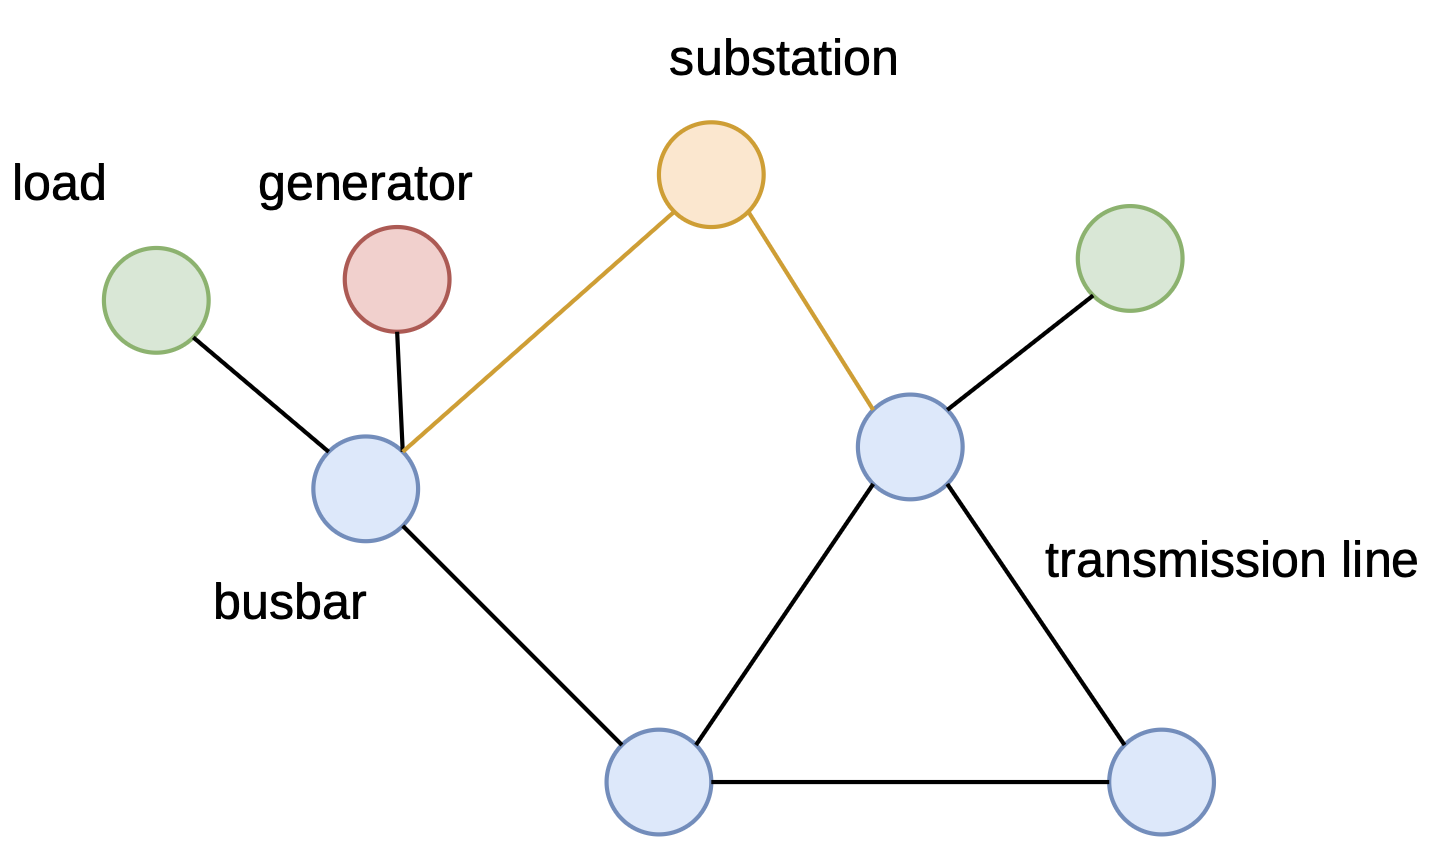
\includegraphics[width=\linewidth]{figures/graph_substation_summary_node.png}
    \caption{Disaggregated graph.}
    \label{fig:substation-summary-node-hetero}
  \end{subfigure}
  \caption{Learned substation-summary augmentation, shown in the two schemas of
  Section~\ref{sec:graph-representation}. The orange substation node receives
  messages from each of its blue busbar nodes and redistributes the resulting
  substation-level representation through the reverse edges. In~(a) the generator and load
  quantities are aggregated into the busbar features, whereas in~(b) they are
  separate nodes; in both cases the summary node attaches only to busbars, so
  generators, loads, and transmission-line nodes reach it through their busbar
  attachments.}
  \label{fig:substation-summary-node}
\end{figure}

\noindent After the raw node projection in
Figure~\ref{fig:graph-actor-pipeline}, the model initializes $u_s$ from a
\emph{structural descriptor} of substation $s$ rather than from its identity.
Let $\boldsymbol\phi_s\in\mathbb R^{4}$ collect the number of busbars, incident
lines, attached generators, and attached loads of that substation, each divided
by a constant that is the same on every grid. The summary node starts at
\begin{equation}
  u_s^{(0)} = \mathbf W_{\mathrm{sub}}\,\boldsymbol\phi_s + \mathbf b_{\mathrm{sub}},
  \qquad
  \mathbf W_{\mathrm{sub}}\in\mathbb R^{d_h\times 4},\;
  \mathbf b_{\mathrm{sub}}\in\mathbb R^{d_h},
  \label{eq:substation-summary-init}
\end{equation}
and carries no current grid measurement. Messages from the busbars then produce
an observation-dependent state for $u_s$, while PPO learns
$\mathbf W_{\mathrm{sub}}$ and $\mathbf b_{\mathrm{sub}}$ with the other
parameters.
\\
\\
{\color{clarif}
The descriptor replaces what would be the obvious construction, a trainable
matrix $\mathbf Q\in\mathbb R^{S\times d_h}$ whose row $s$ is selected by
substation identifier. That version cannot cross grids: its first dimension is
the number of substations, so a checkpoint trained on a $14$-substation network
carries a $14\times d_h$ matrix that no $36$-substation model can accept.
Transfer does not degrade quietly in that case, it stops -- the loader treats
the mismatch as an architecture difference and refuses, since the shape is not
one of the graph-describing buffers it is allowed to rebuild. The augmentation
would therefore have been unusable in exactly the setting
Chapter~\ref{ch:wcci-transfer} is about, and a design screened on
\texttt{bus14} could not have been carried to the larger grid.
\\
\\
Equation~\ref{eq:substation-summary-init} removes that, because both learned
tensors are shaped by the descriptor and not by the network. It also keeps what
the identity version was useful for. The bias $\mathbf b_{\mathrm{sub}}$ is a
single vector shared by every substation, which is what an identity-free design
would give on its own; the weight $\mathbf W_{\mathrm{sub}}$ adds a modulation
by what the substation is made of, so a busy junction and a radial end point do
not start from the same state. The quantities involved are counts rather than
physical magnitudes, so the same descriptor means the same thing on any network,
which is what makes the projection transferable at all.
}

\begin{table}[H]
  \centering
  \small
  \caption{Node and edge features introduced by the substation-summary
  augmentation. Here $d_h$ is the hidden node width; $d_h=128$ in the screened
  GINE models.}
  \label{tab:summary-node-augmentation-features}
  \setlength{\tabcolsep}{4pt}
  \begin{tabular}{L{0.20\textwidth}L{0.31\textwidth}L{0.39\textwidth}}
    \toprule
    Graph schema & Added summary-node state & Feature values on $i\leftrightarrow u_s$ \\
    \midrule
    Busbar & $\mathbf W_{\mathrm{sub}}\boldsymbol\phi_s+\mathbf b_{\mathrm{sub}}\in\mathbb{R}^{d_h}$, from the substation's structural descriptor; no measured feature. & \texttt{rho}$=1$; all other physical-line features are $0$. \\
    Disaggregated & Same structural projection; no measured feature. & \texttt{rho}$=1$; all physical and relation entries are otherwise $0$. \\
    Disaggregated with line nodes & Same structural projection; no measured feature. & All nine relation entries are $0$. \\
    \bottomrule
  \end{tabular}
\end{table}

\noindent In runs with mean readout, each $u_s$ is marked as a valid node and is
included once in the mean together with all other valid nodes. In runs with a virtual
node, there is no terminal mean: the virtual node connects to the summary nodes,
and its final state is used as the graph representation.
\\
\\
The summary-node and direct-edge augmentations may also be enabled together,
and either may be combined with the virtual-node readout.


\section{Pooling and Graph Readout}
\label{sec:graph-pooling}

The final graph embedding is obtained either by pooling node embeddings directly
or by reading out a learned virtual node. The output projection and action head
are the same in both cases.

\subsection{Mean, maximum, and sum pooling}
\label{subsec:graph-mean-pooling}

Mean pooling averages the final embeddings of the valid nodes:
\begin{equation}
  \overline{\mathbf{h}}_G =
  \frac{\sum_v m_v\mathbf{h}^{(K)}_v}
       {\max(1,\sum_v m_v)},
  \label{eq:methods-mean-pooling}
\end{equation}
where $m_v=n^{(a)}_{v,t}$ is the visibility mask. A single mean is computed over
all visible node types; there is no separate pooling operation for each type.
An inactive fixed-shape candidate contributes neither an embedding to the
numerator nor one unit to the denominator. The mask is therefore an additional
enforcement of the construction boundary, not an averaging of zero
placeholders.
\\
\\
Maximum pooling instead selects the largest value independently in every hidden
feature channel:
\begin{equation}
  \left(\overline{\mathbf{h}}^{\max}_G\right)_c =
  \max_{v\,:\,m_v=1}\left(\mathbf{h}^{(K)}_v\right)_c.
  \label{eq:methods-max-pooling}
\end{equation}
It therefore keeps the strongest activation in each channel without depending
on the number of nodes, but it does not preserve how many nodes produced a
similar activation.
\\
\\
Sum pooling is available but is not used in any reported experiment. Its
magnitude grows with the number of nodes. That number differs across agents,
graph representations, and grids, so the scale of a sum-pooled embedding would
also change across the transfer studied in Chapter~\ref{ch:wcci-transfer}.
\\
\\
For ordinary mean, maximum, or sum pooling, the pooled set is every
\emph{visible} node in the agent's local graph. It contains controlled nodes,
including empty controlled busbars and disconnected controlled assets; the
currently connected far-end busbars in \texttt{bus} and
\texttt{heterogeneous}; and all boundary/internal line nodes in
\texttt{heterogeneous\_line}. It never contains an inactive contextual
candidate, a neighboring private asset, or any neighboring equipment in the
explicit-line schema. Valid substation-summary nodes are included when that
augmentation is enabled. Direct same-substation edges add no nodes and do not
change the pooled set.
\\
\\
The alternatives \texttt{controlled\_mean}, \texttt{controlled\_sum}, and
\texttt{controlled\_max} restrict terminal readout to the action domain. For
controlled mean, define $q_v=m_vc_v$, where $c_v$ is the static
\texttt{controlled\_node\_mask}; then
\begin{equation}
  \overline{\mathbf{h}}^{\mathrm{ctrl}}_G =
  \frac{\sum_v q_v\mathbf{h}^{(K)}_v}
       {\max(1,\sum_v q_v)}.
  \label{eq:methods-controlled-mean-pooling}
\end{equation}
Contextual busbars can still affect the controlled embeddings through active
message-passing paths, but do not enter the final aggregation directly. The
controlled pooled set is fixed for an episode, whereas the ordinary visible
set can change when a neighboring line switches busbar or goes offline. This
stabilizes the denominator, but it is a readout choice rather than the leakage
fix: the graph construction and visibility masks enforce the information
boundary for every pooling mode.
\\
\\
The optional \texttt{energized\_mean} readout further requires a node to be
incident to an active electrical relation; self and same-substation relations
do not qualify. \texttt{controlled\_energized\_mean} additionally intersects
this dynamic mask with the controlled-node mask. These masks affect only the
terminal mean and its denominator, not message passing. They are therefore
pooling ablations, not leakage fixes. Virtual-node runs do not use terminal
pooling and are described in Section~\ref{sec:virtual-node-readout}.

{\color{clarif}
\paragraph{Which of the four is the defensible default.}
The readout produces the single vector the action head reads, and in the
candidate-scoring head it is the global context concatenated to every action.
It should therefore answer one question: what is the state of the region this
agent is deciding about? That region is the action domain, which makes
\texttt{controlled\_mean} the appropriate default. Excluding context from the
average does not discard it, because it arrives through message passing, which
is what the graph is for: on a three-substation fixture the
\texttt{controlled\_mean} embedding differs across topologies that differ only
in their context. The choice is not whether context informs the summary but
whether it does so as structure or as an addend, and structure is the answer
that uses the model rather than bypassing it.
\\
\\
The mechanical argument is the stronger one. A fixed pooled set makes any
systematic offset -- including the zeros contributed by empty controlled
busbars -- a constant that the readout projection absorbs during training. A
pooled set whose size moves turns that offset into a quantity varying with
topology, which the network must then separate from genuine signal. On agent
$0$ of \texttt{bus14} the visible set holds ten nodes under the nominal
topology, eleven once a contextual substation splits, and nine after a boundary
line trips, so an ordinary mean rescales every node it keeps when a
\emph{neighbouring} agent acts.
\\
\\
The energised variants are the least defensible of the four, because they
remove precisely what actions target. Four of agent $0$'s eight busbars are
de-energised under the nominal topology: the empty second busbar of each
substation, which is the busbar a splitting action moves an element onto. A
readout that drops them cannot represent the availability of a free busbar,
which is the most directly actionable fact in the observation, and its
denominator moves with every switch.
\\
\\
Two qualifications. When one-hop context is disabled the controlled and visible
sets coincide, so the distinction is vacuous and the ordinary readout is already
the controlled one. And maximum pooling is less exposed throughout: it does not
depend on the size of the pooled set, and a de-energised row of zeros seldom
wins a maximum, so the energised variants matter far less there. Its own risk is
different -- with context included, a neighbour under greater stress dominates
the channel maxima, so the graph summary reports the neighbour's worst channel
rather than the agent's, which is an argument for \texttt{controlled\_max} on the
same grounds.
\\
\\
This also sharpens the reason sum pooling is set aside. The objection above is
that its magnitude follows the number of pooled nodes, and under a controlled
readout that number is fixed for the episode, so the objection would dissolve.
What remains is that the controlled sets differ \emph{between} agents -- eight,
eight and twelve busbars on \texttt{bus14} -- while the encoder is shared, so a
sum would hand different agents systematically different magnitudes.
}

\subsection{Virtual-node graph readout}
\label{sec:virtual-node-readout}

A virtual-node readout replaces terminal mean, sum, maximum, or attention
pooling with one learned graph-summary node. It can be combined with any of the
three graph schemas.

\subsubsection{Augmented graph}
\label{subsec:virtual-node-augmented-graph}

Let $v_{\star}$ denote the virtual node. Define the summary set
$\mathcal{V}_{\mathrm{sum}}$ as the included substation nodes when the
augmentation from Section~\ref{sec:substation-summary-nodes} is enabled, and as
the included busbar nodes otherwise. The augmented graph is
\begin{align}
  \mathcal{V}^{+} &= \mathcal{V}\cup\{v_{\star}\}, \\
  \mathcal{E}^{+} &= \mathcal{E}\cup
  \left\{
    (i,v_{\star})
    \;\middle|\;
    i\in\mathcal{V}_{\mathrm{sum}}
  \right\}.
  \label{eq:virtual-node-augmentation}
\end{align}
All reported experiments use a toward-summary direction: every added edge
points from a node in $\mathcal{V}_{\mathrm{sum}}$ to $v_{\star}$. The virtual
node therefore receives information but never sends messages back. It connects
to all visible busbars, or to all visible substation-summary nodes when that
augmentation is enabled, and has no direct edge to generator, load, or
transmission-line nodes. Candidate virtual edges incident to an inactive
contextual row are masked, so the virtual readout cannot bypass the local
information boundary.

\begin{figure}[htbp]
  \centering
  \begin{subfigure}[b]{0.49\linewidth}
    \centering
    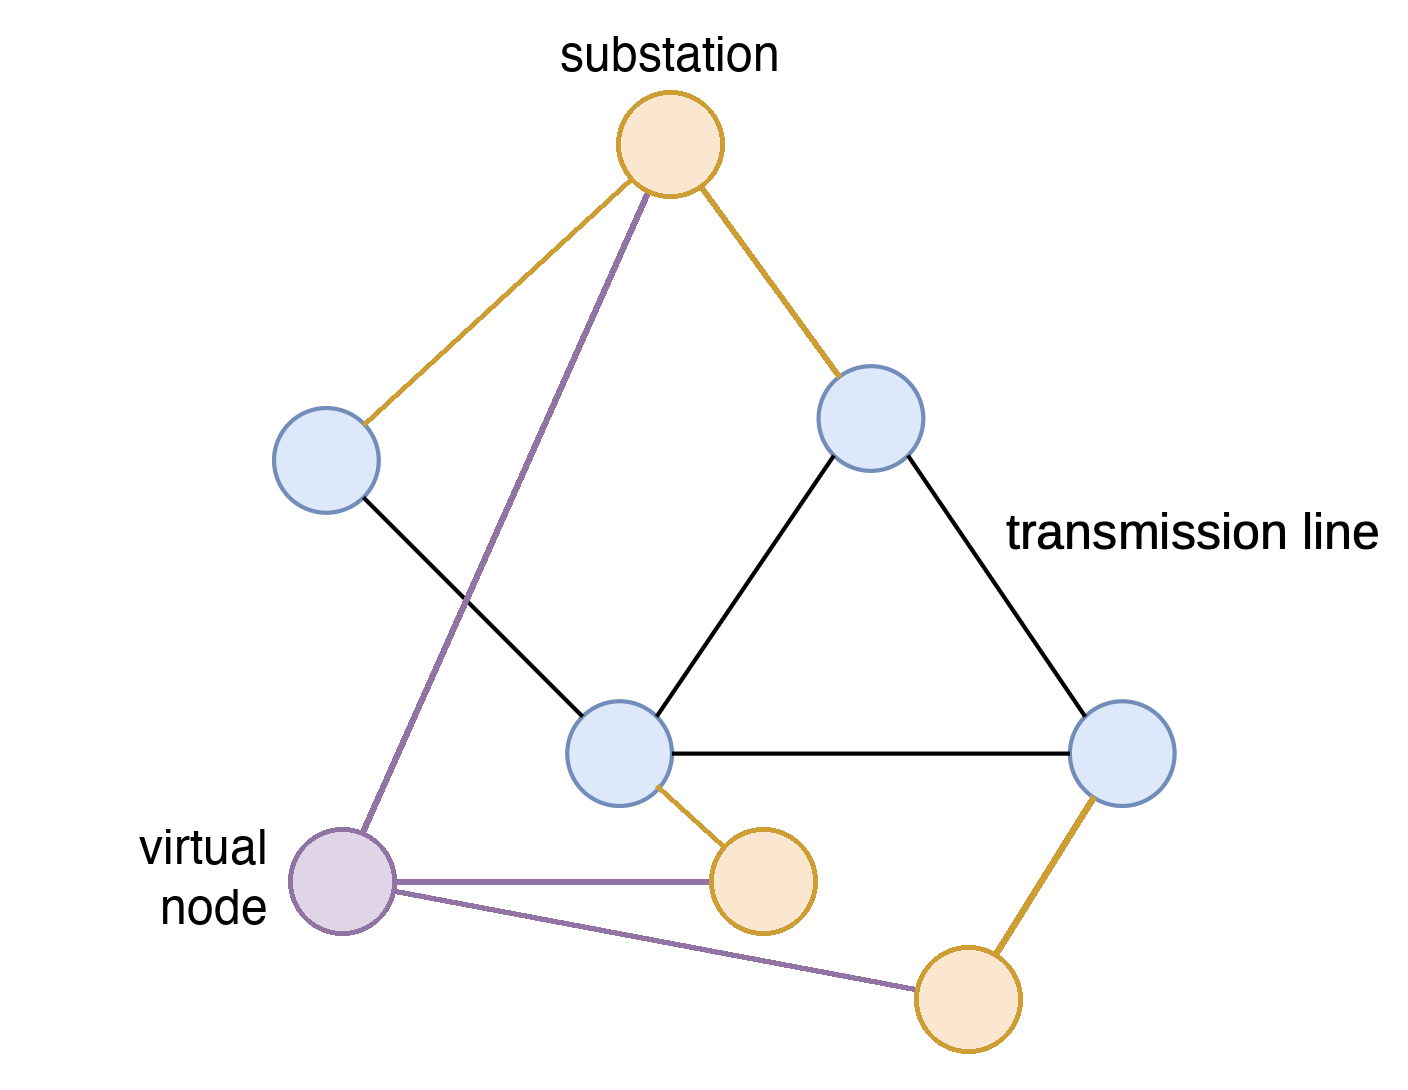
\includegraphics[width=\linewidth]{figures/graph_virtual_node_readout_bus.png}
    \caption{With substation-summary nodes.}
    \label{fig:virtual-node-readout-summary}
  \end{subfigure}
  \hfill
  \begin{subfigure}[b]{0.49\linewidth}
    \centering
    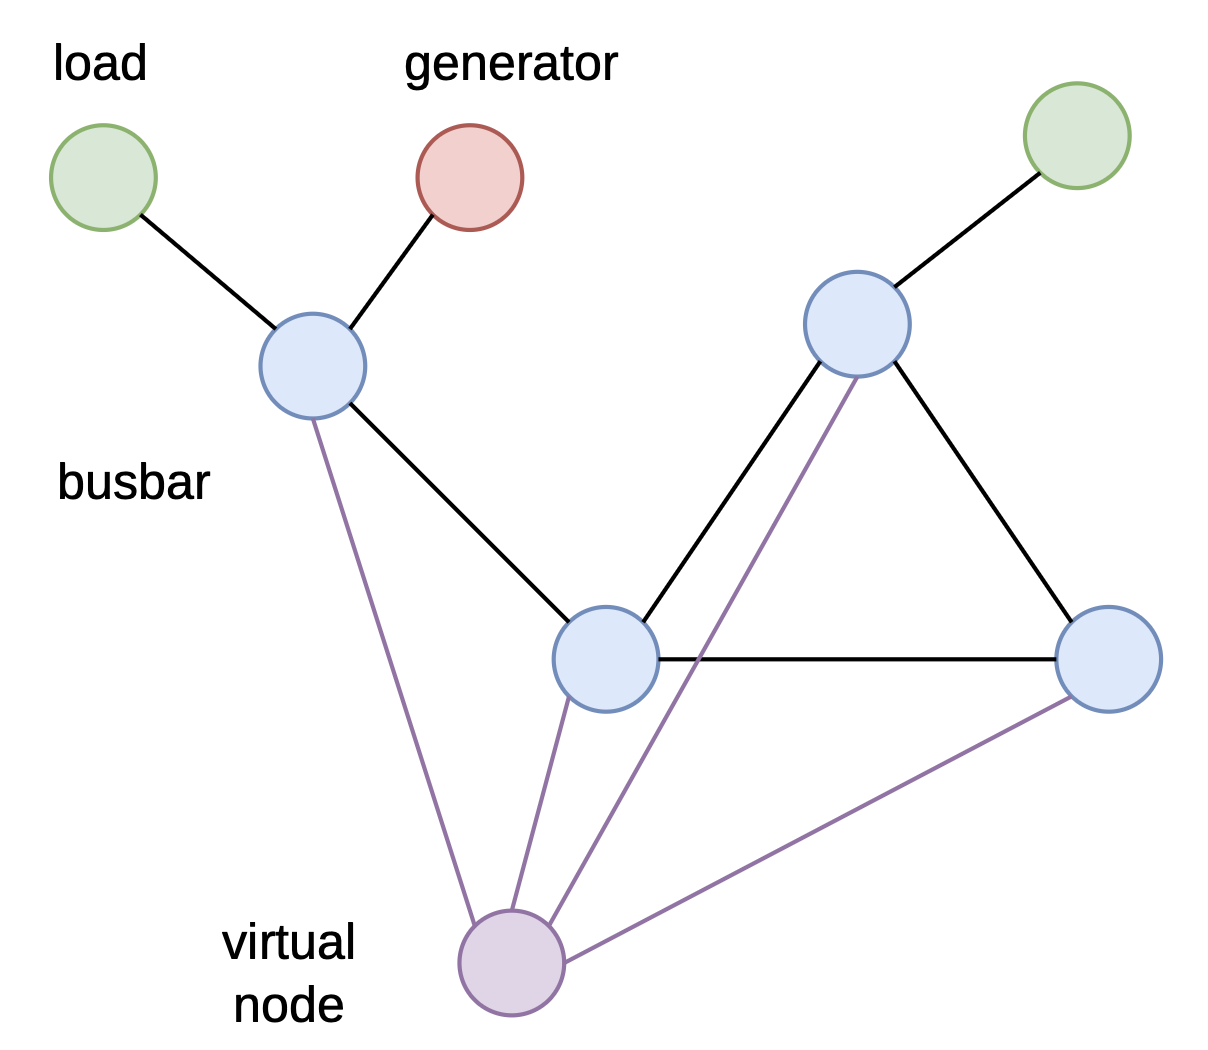
\includegraphics[width=\linewidth]{figures/graph_virtual_node_readout.png}
    \caption{Without substation-summary nodes.}
    \label{fig:virtual-node-readout-busbar}
  \end{subfigure}
  \caption{Virtual-node graph readout, shown for both definitions of the
  summary set $\mathcal{V}_{\mathrm{sum}}$ in
  Equation~\ref{eq:virtual-node-augmentation}. The purple node aggregates that
  set and its final embedding replaces terminal node pooling. Every purple edge
  is directed toward the virtual node, which sends no message back. In~(a) the substation-summary augmentation of
  Section~\ref{sec:substation-summary-nodes} is enabled, so the virtual node
  attaches to the orange substation nodes and reaches the busbars only through
  them, which gives a two-level hierarchy busbar $\rightarrow$ substation
  $\rightarrow$ virtual node. In~(b) the augmentation is disabled and the
  virtual node attaches directly to every included busbar. In neither case does
  it connect to generator, load, or transmission-line nodes.}
  \label{fig:virtual-node-readout}
\end{figure}

\subsubsection{Learned summary instead of terminal pooling}
\label{subsec:virtual-node-summary}

The initial virtual representation $\mathbf{h}_{\star}^{(0)}$ is learned. A
message-passing layer jointly updates the physical and virtual nodes:
\begin{equation}
  \left(
    \{\mathbf{h}_{i}^{(k+1)}\}_{i\in\mathcal{V}},
    \mathbf{h}_{\star}^{(k+1)}
  \right)
  =
  \operatorname{GNN}^{(k)}
  \left(
    \{\mathbf{h}_{i}^{(k)}\}_{i\in\mathcal{V}},
    \mathbf{h}_{\star}^{(k)},
    \mathcal{E}^{+}
  \right).
  \label{eq:virtual-node-update}
\end{equation}
Because every virtual edge points toward $v_{\star}$, it only aggregates the
node states and cannot influence them during message passing. After $K$ layers,
the graph embedding is
\begin{equation}
  \mathbf{z}_{G}
  = \operatorname{ReLU}
    \left(\mathbf{W}_{o}\mathbf{h}_{\star}^{(K)}+\mathbf{b}_{o}\right),
  \label{eq:virtual-node-readout}
\end{equation}
rather than from
$\operatorname{Pool}(\{\mathbf{h}_{i}^{(K)}\}_{i\in\mathcal{V}})$. The output
dimension is unchanged.

\subsubsection{Relation attributes and encoder compatibility}
\label{subsec:virtual-node-compatibility}

Virtual connections are structural: their continuous edge attributes are zero,
except for a neutral unit value in the
\texttt{rho} position when that feature exists.
\\
\\
Without substation nodes, a graph containing $N_{\mathrm{bus}}$ included
busbars receives one virtual node and $N_{\mathrm{bus}}$ directed edges. With
the hierarchy enabled, the virtual-node stage instead adds $S$ edges from the
$S$ substation-summary nodes. After one layer the virtual node has aggregated
its immediate busbar or substation neighbors.

\begin{tcolorbox}[
  colframe=red!75!black,
  colback=red!5!white,
  title=Chapter Summary (2/3): Augmentations and Graph Readout
]
\textbf{Purpose:} Separate changes to information exchange inside the graph
from changes to the final graph-level representation.

\begin{itemize}
  \item \textbf{Direct substation edges ($e$):} Add structural relations between
  busbars of the same substation, without adding nodes or representing a
  physical transmission line.
  \item \textbf{Substation nodes ($n$):} Add one learned node per substation.
  It has no raw electrical measurement, is updated from its busbars, and can be
  included in the graph readout.
  \item \textbf{Terminal pooling:} Ordinary mean pooling averages every visible
  node, including electrically connected contextual busbars and valid added
  substation nodes; masked contextual candidates are excluded. A
  \texttt{controlled\_*} readout instead aggregates only the fixed action-domain
  nodes, while still allowing visible context to influence them through message
  passing. Maximum pooling keeps the largest value in each hidden channel. Sum
  pooling is not used because its scale changes with the number of nodes.
  \item \textbf{Virtual readout ($v$):} Replace terminal pooling with one learned
  grid-summary node. Messages travel only toward this node, from the busbars or
  from the added substation nodes, and its final state becomes the graph
  embedding.
\end{itemize}

\textbf{Takeaway:} Factors $e$ and $n$ modify message passing, whereas pooling
and factor $v$ determine how the encoded local graph is reduced to one vector
for action selection. These choices can be combined with any base graph schema.
\end{tcolorbox}

\section{Candidate-Action Scoring from the Explicit-Line Graph}
\label{sec:candidate-action-scoring}

The default action head produces one output column per discrete action. That
column is tied to an action index and knows nothing about the physical objects
the action modifies. This section describes an alternative head that scores each
action from the graph nodes it touches. It is available only for the
explicit-line schema of Section~\ref{sec:heterogeneous-line-graph} and is
selected with \texttt{actor\_action\_head=candidate\_pool}; the default remains
the action-index head of Appendix~\ref{sec:gnn-action-head}. The PPO objective,
the categorical policy, sampling, and deterministic evaluation are unchanged.

\subsection{From action indices to candidate scoring}
\label{subsec:candidate-motivation}

Throughout this section, $\mathbf{z}_a$ denotes the graph embedding of agent
$a$: the node states of its local graph pooled as in
Section~\ref{sec:graph-pooling} and passed through the output projection
(Equation~\ref{eq:gnn-output-projection}). It is one 128-dimensional vector per
agent per step, and it is the only thing the actor has ever seen of the graph.
\\
\\
With the default head, agent $a$ produces its logit vector in one step from
$\mathbf{z}_a$:
\begin{equation}
  \boldsymbol{\ell}_a = \operatorname{MLP}_a(\mathbf{z}_a),
  \qquad \boldsymbol{\ell}_a\in\mathbb{R}^{|\mathcal{A}_a|}.
  \label{eq:action-index-head}
\end{equation}
The last layer has one row per action index, so what makes an action good must
be learned separately for every index, and the head grows with
$|\mathcal{A}_a|$.
\\
\\
Candidate scoring replaces that by one shared scalar-valued network applied to
every action in turn:
\begin{equation}
  \ell_{a,j} =
  \operatorname{score}
  \left(
    \underbrace{\mathbf{z}_a}_{\text{whole graph}},\
    \underbrace{\mathbf{c}_j}_{\text{nodes action }j\text{ touches}},\
    \underbrace{\boldsymbol{\phi}_j}_{\text{what action }j\text{ does}}
  \right).
  \label{eq:candidate-scoring-head}
\end{equation}
The same parameters score all actions, so the head no longer grows with
$|\mathcal{A}_a|$, and two actions are ranked by the difference between their
touched-node contexts rather than by two independent output rows. This is what
makes the explicit line nodes usable: an action next to a loaded line is scored
from that line's own embedding.
\\
\\
Two ingredients are needed: a static table saying which nodes each action
touches (Section~\ref{subsec:candidate-action-metadata}), and a rule for
turning those nodes into the context vector $\mathbf{c}_j$
(Section~\ref{subsec:candidate-pooling}).

\subsection{What each action touches}
\label{subsec:candidate-action-metadata}

The first ingredient is one lookup table per agent, with one row per action,
answering a single question: which nodes of the local graph does this action
physically touch? It is built once, when the environment is created, and never
recomputed during training.
\\
\\
A Grid2Op topology action states which entries of the topology vector it
changes, and each entry belongs to a known object: a line endpoint, a
generator, or a load. Reading those entries gives the objects the action
modifies, and the graph builder's row maps turn each object into the row of the
graph that holds its embedding. Table~\ref{tab:candidate-metadata-example}
follows one action through this.

\begin{table}[H]
  \centering
  \small
  \caption{One action, from Grid2Op to node rows: moving the origin end of
  line~4 onto the other busbar of substation~6. Row indices are illustrative.}
  \label{tab:candidate-metadata-example}
  \setlength{\tabcolsep}{5pt}
  \begin{tabular}{L{0.28\textwidth}L{0.62\textwidth}}
    \toprule
    Step & Result for this action \\
    \midrule
    Objects the action changes & Substation 6, line 4 \\
    Their rows in the graph & Both busbars of substation 6, here 12 and 13, and the line node of line 4, here 22 \\
    Stored for scoring & Busbar $[12,13]$, line $[22]$, generator and load empty \\
    \bottomrule
  \end{tabular}
\end{table}

\noindent Two decoding rules are worth stating. A touched substation contributes
\emph{all} of its busbar rows, not only the busbar in use, because the action
changes which of them the equipment sits on. A boundary line contributes its
explicit line-node row and the controlled endpoint rows that are present in the
local graph; scoring does not add the far-end busbar or any neighboring private
asset. The rows are stored as fixed-size arrays with a mask, padded to the
widest action, so that a single gather serves the whole action space.
\\
\\
Write $\mathcal{N}_{\mathrm{bus}}(j)$, $\mathcal{N}_{\mathrm{line}}(j)$,
$\mathcal{N}_{\mathrm{load}}(j)$, and $\mathcal{N}_{\mathrm{gen}}(j)$ for the
four sets of node rows that action $j$ touches. Because a topology change moves
line endpoints, the explicit line node must be present whenever the line
touches the agent's controlled domain. The leakage-free construction guarantees
that membership without constructing the non-controlled endpoint.
\\
\\
Each action also carries a static feature vector
$\boldsymbol{\phi}_j\in\mathbb{R}^{12}$, listed in
Table~\ref{tab:candidate-action-features}. It describes what the action does
independently of the current grid state, so the scorer can tell a single
endpoint move from an action that reconfigures a whole substation even when
both touch the same nodes.

\begin{table}[H]
  \centering
  \small
  \caption{The static action-feature vector $\boldsymbol{\phi}_j$. The five
  indicators are binary; the seven counts are divided by their largest value
  over that agent's action space, so every entry lies in $[0,1]$ and is
  independent of the grid size.}
  \label{tab:candidate-action-features}
  \setlength{\tabcolsep}{5pt}
  \begin{tabular}{L{0.36\textwidth}L{0.54\textwidth}}
    \toprule
    Entry & Meaning \\
    \midrule
    \multicolumn{2}{l}{\emph{Indicators}} \\
    \texttt{is\_do\_nothing} & The action is the idle action \\
    \texttt{has\_busbar\_context} & It modifies at least one substation \\
    \texttt{has\_line} & It touches at least one line \\
    \texttt{has\_load} & It touches at least one load \\
    \texttt{has\_generator} & It touches at least one generator \\
    \midrule
    \multicolumn{2}{l}{\emph{Scaled counts}} \\
    \texttt{n\_substations} & Substations modified \\
    \texttt{n\_topology\_changes} & Topology-vector entries changed \\
    \texttt{n\_line\_status\_changes} & Lines connected or disconnected \\
    \texttt{n\_line\_endpoint\_changes} & Line endpoints moved to another busbar \\
    \texttt{n\_generator\_changes} & Generators moved to another busbar \\
    \texttt{n\_load\_changes} & Loads moved to another busbar \\
    \texttt{n\_other\_changes} & Changed objects of any other type \\
    \bottomrule
  \end{tabular}
\end{table}

\subsection{Pooling the touched nodes}
\label{subsec:candidate-pooling}

The second ingredient turns the touched rows into $\mathbf{c}_j$. In
$\mathbf{z}_a$ the nodes have already been averaged away, so the encoder also
returns the node states themselves:
\begin{equation}
  (\mathbf{z}_a,\mathbf{H})
  = \operatorname{encoder}_{\mathrm{nodes}}(\mathcal{G}^{(a)}_t),
  \qquad
  \mathbf{H}\in\mathbb{R}^{|\mathcal{V}|\times d_h},
  \label{eq:forward-with-nodes}
\end{equation}
where row $v$ of $\mathbf{H}$ is the state $\mathbf{h}^{(K)}_v$ of node $v$
after the last message-passing layer. These are exactly the vectors that mean
pooling averages into $\mathbf{z}_a$; nothing new is computed, and a run with
the default head is unaffected. Only the physical nodes appear in $\mathbf{H}$:
substation-summary and virtual nodes are excluded, since an action touches
equipment and not a learned hub.
\\
\\
The basic operation is a masked mean over the rows of one object type,
\begin{equation}
  \mathbf{c}^{(t)}_j =
  \frac{1}{\max\left(1,|\mathcal{N}_t(j)|\right)}
  \sum_{v\in\mathcal{N}_t(j)}\mathbf{h}^{(K)}_v,
  \label{eq:candidate-typed-mean}
\end{equation}
where the clamped denominator makes an untouched type give the zero vector
instead of a division by zero. Table~\ref{tab:candidate-pool-modes} lists the
ways of combining these.

\begin{table}[H]
  \centering
  \small
  \caption{Pooling modes. All three are implemented; \texttt{typed\_mean} is the
  default.}
  \label{tab:candidate-pool-modes}
  \setlength{\tabcolsep}{5pt}
  \begin{tabular}{L{0.17\textwidth}L{0.36\textwidth}L{0.10\textwidth}L{0.27\textwidth}}
    \toprule
    Mode & Context $\mathbf{c}_j$ & Width & What it buys \\
    \midrule
    \texttt{mean} & One masked mean over all touched rows, whatever their type & $d_h$ & The smaller control; mixes roles together \\
    \texttt{typed\_mean} & The four typed means of Equation~\ref{eq:candidate-typed-mean}, concatenated & $4d_h$ & The scorer can tell a stressed line from the load beside it \\
    \texttt{typed\_attention} & The action queries the eligible rows and weights them, typed as above & $4d_h$ & Can focus on the one endpoint that matters instead of averaging it away \\
    \bottomrule
  \end{tabular}
\end{table}

\noindent Learned attention replaces the flat average by weights the action computes for
itself, and \texttt{candidate\_action\_attention\_scope} decides which rows
compete for that weight: \texttt{affected} keeps the touched rows of the two
means above, \texttt{all} opens the attention to every node of the local graph,
and \texttt{soft\_prior} opens it to every node but biases the touched ones,
so the head can look beyond what the action modifies without being forced to.
The uniform modes are still the controls, because attention adds parameters and
a second failure mode to a head whose value is being established at the same
time.

\subsection{Scoring, including the idle action}
\label{subsec:candidate-scorer}

All non-idle actions are scored by one network with a single output unit:
\begin{equation}
  \ell_{a,j} =
  \operatorname{MLP}_{\mathrm{score}}
  \left(
    \left[\mathbf{z}_a;\mathbf{c}_j;\boldsymbol{\phi}_j\right]
  \right),
  \qquad j\geq 1.
  \label{eq:candidate-shared-scorer}
\end{equation}
The idle action touches nothing, so its pooled context is identically zero and
would otherwise be scored by a network trained on non-zero contexts. It
therefore gets its own head over the graph embedding alone:
\begin{equation}
  \ell_{a,0} =
  \operatorname{MLP}_{\varnothing}(\mathbf{z}_a) + b_{\varnothing},
  \label{eq:candidate-do-nothing-head}
\end{equation}
with $b_{\varnothing}$ a learned scalar applied to action $0$ alone. This makes
the idle logit an explicit judgment of whether the local grid state is safe
enough not to intervene.

{\color{blue}
\subsection{Cost and current limits}
\label{subsec:candidate-configuration}

The candidate contexts form a tensor of shape
$\left[\text{batch},|\mathcal{A}_a|,d_c\right]$, so memory grows with the size
of the action space. This is the reason to start on \texttt{bus14} and on
reduced action spaces before the full WCCI one.
\\
\\
Two properties matter when comparing this head against the default. The head no
longer scales with $|\mathcal{A}_a|$, so the two actors do not have the same
parameter count even at identical graph settings, and both counts should be
reported. The idle logit also comes from a different mechanism than the other
logits, so the action-$0$ frequency has to be compared against the action-index
baseline rather than assumed comparable.
\\
\\
The head currently requires the explicit-line graph and does not combine with
the intervention gate, which is refused at construction rather than silently
ignored. One-hop context is not required, and the experiments of
Section~\ref{sec:line-node-angle} run without it: the neighbor-inclusion setting
adds no far-end equipment to this representation, because the shared-line state
is supplied by the line node itself. Auxiliary heads over the same node
embeddings, such as predicting which lines are about to overload, are a possible
later addition.
}
\section{Action-Space Reduction for Large Grids}
\label{sec:wcci-action-space-reduction}

The representations above change what an agent sees. This section changes what
it can do, and is what makes the larger grids tractable at all: the WCCI bus36
setting has a far larger discrete topology-action space than \texttt{bus14}, so
before training MAPPO on it the action space is reduced offline from simulated
action outcomes. During rollouts, states are collected
when the grid is stressed,
\[
  \rho_{\max}>0.90.
\]
For each collected state \(s\), candidate actions are simulated and compared
against do nothing:
\[
  \Delta(s,a)=\rho_{\mathrm{after}}(s,a)
  -\rho_{\mathrm{after}}(s,0).
\]
An action is counted as useful when it lowers the post-action loading relative
to do nothing, i.e. \(\Delta(s,a)<-\epsilon\). Each action is then scored by its
empirical improvement rate,
\[
  \mathrm{score}(a)=
  \frac{\#\{\text{tested states where }a\text{ improves the grid}\}}
       {\#\{\text{tested states where }a\text{ is evaluated}\}},
\]
with a minimum-count filter to avoid selecting rarely sampled actions. The final
reduced action space keeps the best actions per agent, while always preserving
action \(0\). The candidate sets are then sanity-checked with a one-step
simulator-greedy controller: at each risky state, the controller simulates the
available reduced actions and executes the best improving one. That check also
sizes the reduced space, since it shows how much survival is still reachable
once the action set is cut. Table~\ref{tab:wcci-h1-greedy-reduced-action-spaces}
reports it for five sizes; the survival of trained agents on this environment is
a separate question and is not covered here.

\begin{table}[htbp]
  \centering
  \small
  \caption{One-step greedy evaluation of WCCI reduced action spaces on 50
  random test chronics. All rows use the same chronic sample
  (\texttt{chronic\_sample\_seed=0}); the do-nothing mean survival on this
  sample is \(28.30\%\).}
  \label{tab:wcci-h1-greedy-reduced-action-spaces}
  \setlength{\tabcolsep}{4pt}
  \resizebox{\textwidth}{!}{%
  \begin{tabular}{L{0.30\textwidth}L{0.28\textwidth}rrrr}
    \toprule
    Reduced action space & Kept actions per agent
    \((a_0,a_1,a_2,a_3)\) & Greedy survival (\%) &
    Do-nothing survival (\%) & Survival delta (\%) & Greedy full survival (\%) \\
    \midrule
    Do-nothing reference & \(1,1,1,1\) & -- & 28.30 & -- & -- \\
    WCCI \(h=1\), \texttt{mk64} & \(64,64,64,64\) & 55.24 & 28.30 & 26.94 & 22.00 \\
    WCCI \(h=1\), \texttt{mk128} & \(77,128,127,128\) & 60.65 & 28.30 & 32.35 & 22.00 \\
    WCCI \(h=1\), \texttt{mk256} & \(77,256,127,256\) & 68.61 & 28.30 & 40.31 & 36.00 \\
    WCCI \(h=1\), \texttt{mk512} & \(77,512,127,512\) & 71.21 & 28.30 & 42.90 & 40.00 \\
    WCCI \(h=1\), \texttt{mk1024} & \(77,1024,127,1024\) & 78.18 & 28.30 & 49.87 & 54.00 \\
    \bottomrule
  \end{tabular}
  }
\end{table}

\begin{tcolorbox}[
  colframe=red!75!black,
  colback=red!5!white,
  title=Chapter Summary (3/3): Action Scoring and Large-Grid Reduction
]
\textbf{Purpose:} Define how graph embeddings become action logits and how the
large WCCI action space is made tractable.

\begin{itemize}
  \item \textbf{Default action head:} An agent-specific MLP maps the graph
  embedding directly to one logit per discrete action.
  \item \textbf{Candidate-action head:} The optional explicit-line variant
  scores each non-idle action from the encoded nodes it modifies and from static
  action descriptors. The idle action has a separate score. The PPO objective
  and categorical policy are unchanged.
  \item \textbf{Current scope:} Candidate scoring requires the explicit-line
  graph, and its memory cost still grows with the number of candidate actions.
  One-hop context is optional, since the line node already carries the shared
  measurements.
  \item \textbf{WCCI reduction:} Actions are ranked offline by how often they
  reduce loading in simulated stressed states. Action 0 is always retained, and
  the reduced sets are checked with a one-step simulator-greedy controller
  before policy training.
\end{itemize}

\textbf{Takeaway:} Graph representation, action scoring, and action-space size
are separate design choices. This chapter defines them; the following chapters
evaluate the resulting policies.
\end{tcolorbox}
